% main.tex
%
% LaTeX template for creating an MNRAS paper
%
% v3.0 released 14 May 2015
% (version numbers match those of mnras.cls)
%
% Copyright (C) Royal Astronomical Society 2015
% Authors:
% Keith T. Smith (Royal Astronomical Society)

% Change log
%
% v3.0 May 2015
%    Renamed to match the new package name
%    Version number matches mnras.cls
%    A few minor tweaks to wording
% v1.0 September 2013
%    Beta testing only - never publicly released
%    First version: a simple (ish) template for creating an MNRAS paper

%%%%%%%%%%%%%%%%%%%%%%%%%%%%%%%%%%%%%%%%%%%%%%%%%%
% Basic setup. Most papers should leave these options alone.
\documentclass[fleqn,usenatbib]{mnras}

% MNRAS is set in Times font. If you don't have this installed (most LaTeX
% installations will be fine) or prefer the old Computer Modern fonts, comment
% out the following line
\usepackage{newtxtext,newtxmath}
% Depending on your LaTeX fonts installation, you might get better results with one of these:
%\usepackage{mathptmx}
%\usepackage{txfonts}

% Use vector fonts, so it zooms properly in on-screen viewing software
% Don't change these lines unless you know what you are doing
\usepackage[T1]{fontenc}

% Allow "Thomas van Noord" and "Simon de Laguarde" and alike to be sorted by "N" and "L" etc. in the bibliography.
% Write the name in the bibliography as "\VAN{Noord}{Van}{van} Noord, Thomas"
\DeclareRobustCommand{\VAN}[3]{#2}
\let\VANthebibliography\thebibliography
\def\thebibliography{\DeclareRobustCommand{\VAN}[3]{##3}\VANthebibliography}


%%%%% AUTHORS - PLACE YOUR OWN PACKAGES HERE %%%%%

% Only include extra packages if you really need them. Common packages are:
\usepackage{graphicx}	% Including figure files
\usepackage{amsmath}	% Advanced maths commands
% \usepackage{amssymb}	% Extra maths symbols

%%%%%%%%%%%%%%%%%%%%%%%%%%%%%%%%%%%%%%%%%%%%%%%%%%

%%%%% AUTHORS - PLACE YOUR OWN COMMANDS HERE %%%%%

% Please keep new commands to a minimum, and use \newcommand not \def to avoid
% overwriting existing commands. Example:
%\newcommand{\pcm}{\,cm$^{-2}$}	% per cm-squared

\newcommand{\studentt}[2]{t_\nu \left( #1, #2 \right)}
\newcommand{\depvar}{y_i}
\newcommand{\indepvars}{\boldsymbol{x}_i}
\newcommand{\obsdep}{\hat{y}_i}
\newcommand{\obsindep}{\hat{\boldsymbol{x}}_i}
\newcommand{\indepcov}{\Sigma_{x, i}}
\newcommand{\deperr}{\sigma_{y, i}}
\newcommand{\intscttr}{\sigma_{\text{int}}}
\newcommand{\intercept}{\alpha}
\newcommand{\covariate}{\beta}

%%%%%%%%%%%%%%%%%%%%%%%%%%%%%%%%%%%%%%%%%%%%%%%%%%

%%%%%%%%%%%%%%%%%%% TITLE PAGE %%%%%%%%%%%%%%%%%%%

% Title of the paper, and the short title which is used in the headers.
% Keep the title short and informative.
\title[Robust regression in astronomy]{Robust Bayesian regression in astronomy}

% The list of authors, and the short list which is used in the headers.
% If you need two or more lines of authors, add an extra line using \newauthor
\author[W. Martin \& D. Mortlock]{
William Martin$^{1}$\thanks{E-mail: w.martin19@imperial.ac.uk}
and Daniel Mortlock$^{1,2,3}$
\\
% List of institutions
$^{1}$Department of Physics, Imperial College London, Blackett Laboratory, Prince Consort Road, London SW7 2AZ, UK\\
$^{2}$Department of Mathematics, Imperial College London, London, SW7 2AZ, UK\\
$^{3}$Department of Physics, The Oskar Klein Centre, Stockholm University, Albanova, SE-10691 Stockholm, Sweden
}

% These dates will be filled out by the publisher
\date{Accepted XXX. Received YYY; in original form ZZZ}

% Enter the current year, for the copyright statements etc.
\pubyear{2023}

% Don't change these lines
\begin{document}
\label{firstpage}
\pagerange{\pageref{firstpage}--\pageref{lastpage}}
\maketitle

% Abstract of the paper
\begin{abstract}
A Bayesian hierarchical model for robust linear regression in the presence of measurement error is described.
The performance of the model is assessed on both simulated and real datasets.
The code is made available for others to use.
\end{abstract}

% Select between one and six entries from the list of approved keywords.
% Don't make up new ones.
\begin{keywords}
methods: statistical -- methods: data analysis -- software: data analysis
\end{keywords}

%%%%%%%%%%%%%%%%%%%%%%%%%%%%%%%%%%%%%%%%%%%%%%%%%%

%%%%%%%%%%%%%%%%% BODY OF PAPER %%%%%%%%%%%%%%%%%%

\section{Introduction}
\label{sec:intro}

% {\color{red}

% (Each point is ~1 paragraph.)

% Regression generally important in astronomy (e.g., M-$\sigma$)

% Astronomy data well characterised errors, but with some outliers

% Previously sigma-clipping or outlier removal; better to model the full measurement process

% Review of previous methods (e.g., Kelly)

% Characterise as an example of robust inference (i.e., don't need to know the actual generating distribution); mention some existing uses of this (e.g., Feeney, Park)

% Then say presenting practical methodology and implementation here.
% }

Linear regression is a common problem in astronomy, arising in fields as
diverse as {\color{red} galaxy formation and evolution (e.g. the black hole
mass -- stellar velocity dispersion correlation), stellar physics (e.g. the
Leavitt law linking the luminosity and pulsation period for Cepheid variable
stars), and...}. For this reason, there are a plethora of techniques used by
astronomers for linear regression when both the dependent and independent
variables are measured with error \citep[e.g.][]{Press:1992, Akritas:1996,
Tremaine:2002, Kelly:2007}.

\citet{Kelly:2007} illustrates that common ad-hoc
estimators such as \textsc{fitexy} \citep{Press:1992, Tremaine:2002} and
\textsc{bces} \citep{Akritas:1996} suffer from biases and can underestimate
intrinsic scatter.
Similar algorithms exist for removing
outliers from data \citep[e.g.][Sigma clipping]{xxxx} have been used previously
\citep[e.g.][]{Riess:xxxx}, but these can
lead to controversy \citep[e.g.][]{Efstathiou:2013}. A more principled approach
is to model the entire measurement process.

Bayesian hierarchical models (BHMs) are a natural way to model such datasets ---
this allows astronomers to account for, e.g., measurement errors, selection
effects, interlinked parameters, censored data, and many other effects common to
astronomical problems. BHMs have seen increasing use in astrophysics over the
past 30 years, from the distance-redshift relation in cosmology
\citep[e.g.][]{Feeney:2018, Avelino:2019} and photometric redshift estimation
\citep[e.g.][]{Leistedt:2016} to exoplanet characterisation
\citep[e.g.][]{Sestovic:2018} and population-level inference
\citep[e.g.][]{Kelly:2009} --- see \citet{Feigelson:2021} for a recent review
including further examples of BHMs.

\citet{Kelly:2007} presented a general Bayesian hierarchical
model for linear regression with measurement errors and censored data.
\citeauthor{Kelly:2007} found that the Bayesian approach had several advantages
over the other methods considered: no bootstrapping was required to obtain
uncertainties on parameters; the Bayesian approach was easily extensible to
truncated or censored data; and other methods would sometimes severely
underestimate intrinsic scatter in the data. This formulation of Bayesian
regression, sometimes known as \textsc{linmix\_err}, is now commonly used in
astronomy \citep[e.g.][]{McConnell:2013, Bentz:2013, Andrews:2013}.
% However, the model is designed to be sampled using Gibbs sampling, which limits
% the choice of distributions for variables within the model and the number of
% parameters that can be fit simultaneously.
The model assumes parameters are normally distributed throughout; however,
inference that relies on normal distributions can be unduly affected by outliers
(see Section \ref{sec:results} for an exploration of this effect).

The problem of outliers within datasets can be thought of as model
misspecification: these objects do not fit the distributions used to model them.
The ideas behind robust inference can prove useful for this problem; in robust
inference, methods are designed to work irrespective of the actual generative
distribution {\color{red} \citep{Berger:1994}}. One approach is the use of
Student's $t$-distributions, which are leptokurtic (i.e. have heavier tails than
a normal distribution) and can, therefore, lead to more robust results in the
case of model misspecification \citep[e.g.][]{Berger:1994, Gelman:2013}.
Student's $t$-distributions have seen use in bespoke astronomical
\citep[e.g.][]{Park:2017} and cosmological \citep[e.g.][]{Feeney:2018}
inference, but there is not currently a generic robust method for Bayesian
astronomical data analysis.

We propose a development of a generic approach for robust astronomical data
analysis. From the review of previous methods, we can identify properties that
we would like to see in our regression model:

\begin{itemize}
	\item A Bayesian hierarchical model -- we favour a hierarchical approach
	because it naturally encodes the hierarchical structure of astronomical
	regression problems (i.e.\ objects are drawn from a high-level population;
	the objects intrinsically obey some relationship; the objects are measured
	with error and only the measured values are known). We favour a Bayesian
	approach because it gives posterior distributions encoding our degree of
	belief of the values of parameters, quantifying our uncertainty in their
	values.

	\item A robust model -- we desire a model that is robust to both outliers
	(i.e.\ data points that, whether intrinsically or by virtue of measurement
	errors, do not lie on our regression relation) and model misspecification
	(i.e.\ where the underlying distribution of data does not match up with the
	distribution assumed for modelling).

	\item A general method -- we seek a model that does not require case-by-case
	optimisation for application to different regression problems (e.g.\ no
	manual outlier identification and removal, no need to rescale prior
	distributions for different problems, etc.)
\end{itemize}

We implement these ideas in this paper, beginning with a discussion of our model
in Section \ref{sec:formalism}. In Section \ref{sec:methods}, we outline the
methods that we use to validate our model; the results of these validation
checks are presented in Section \ref{sec:results}. In Section
\ref{sec:real-world}, we compare the performance of our model on real-world
datasets with the models outlined in \citet{Kelly:2007} and \citet{Park:2017},
before concluding remarks in Section \ref{sec:conclusions}.

\section{Formalism}
\label{sec:formalism}

In this section, we establish notation and set out our model. We
have $N$ objects, each with some associated independent quantities
$\{\boldsymbol{x}_i\}$ and a dependent quantity $\{y_i\}$. We assume that these
quantities are related by the equations
\begin{align}
    y_i =&\; f(\boldsymbol{x}_i; \boldsymbol{\theta}_f) + \epsilon_i, \\
    \epsilon_i \sim&\; \mathcal{P}_{\text{int}} \left( \boldsymbol{\theta}_{\text{int}} \right),
\end{align}
where $f(\boldsymbol{x}_i; \boldsymbol{\theta}_f)$ is a function relating
$\{\boldsymbol{x}_i\}$ to $\{y_i\}$, with parameters $\boldsymbol{\theta}_f$,
and $\mathcal{P}_{\text{int}}$ is an unknown probability distribution with
parameters $\boldsymbol{\theta}_{\text{int}}$.

These objects are then observed by astronomers, resulting in the measured
data
\begin{align}
    \hat{\boldsymbol{x}}_i =&\; \boldsymbol{x}_i + \boldsymbol{\epsilon}_{x,i}, \\
    \hat{y}_i =&\; y_i + \epsilon_{y,i}, \\
    \boldsymbol{\epsilon}_{x,i} \sim&\; \mathcal{P}_{\text{obs}} \left( \boldsymbol{\theta}_{\text{obs}} \right), \\
    \epsilon_{y,i} \sim&\; \mathcal{P}_{\text{obs}} \left( \boldsymbol{\theta}_{\text{obs}} \right),
\end{align}
where $\mathcal{P}_{\text{obs}}$ is an unknown probability distribution with
parameters $\boldsymbol{\theta}_{\text{obs}}$.

In a Bayesian framework, we can extend this model to deal with, e.g., censored
data or selection effects, but this is beyond the scope of the current work ---
see \citet{Kelly:2007} for an overview of an approach that would incorporate
these effects.

\subsection{Building a robust model}
\label{sec:formalism.robust}

In the setup outlined above, we do not know what the distributions
$\mathcal{P}_{\text{int}}$ and $\boldsymbol{\theta}_{\text{obs}}$ are. A common
assumption in analysis is to use normal distributions to model both of these
distributions. However, in the case of model misspecification (where, e.g., we
assume $\mathcal{P}_{\text{int}}$ is a normal distribution but it is a different
distribution), the results obtained under this assumption can be biased.
Making the assumption that $\mathcal{P}_{\text{int}}$ follows a different
distribution, such as a Student's $t$-distribution \citep{??} or a Gaussian
mixture model \citep{??}, can give results that are robust to this model
misspecification. This means that, even though we do not believe that the
distribution we choose to model $\mathcal{P}_{\text{int}}$ is the same as the
underlying, unknown $\mathcal{P}_{\text{int}}$, we can be confident in the
results achieved.

In this paper, we use Student's $t$-distributions to build a model that is
robust to model misspecification.

\subsection{Sampling distribution}
\label{sec:formalism.sampling}

Student's $t$-distributions are encountered when estimating the mean of a normal
distribution with unknown variance from a limited number of samples. The number
of samples is a parameter of the distribution: for $n$ samples, the
corresponding Student's $t$-distribution will have $\nu \equiv n - 1$
``degrees-of-freedom''. This value of $\nu$ parameterises how heavy-tailed the
distribution is. While the interpretation of $\nu$ as ``degrees-of-freedom''
only makes sense for $\nu \in \mathbb Z^+$, the distribution is normalisable for
any positive, real $\nu$; for this reason, we shall refer to $\nu$ as the shape
parameter.
% Constructing a statistical model that treats this shape parameter as
% a free parameter to be fitted allows the model to adapt to outliers in the data,
% reverting to the result of a model that uses normal distributions in the absence
% of outliers \citep{Feeney:2018}. In this context, $\nu$ is considered a
% nuisance parameter: its exact value is unimportant, and its inclusion in the
% model is solely to ensure that inference is robust to outliers.

The Student's $t$-distribution, with location $\mu$ and scale $\sigma$, has
the probability density function
\begin{equation}
    t_{\nu} \left(x; {\mu}, {\sigma}\right)
        =
    \frac{1}{\sqrt{\pi \nu} \sigma}
    \frac{
        \Gamma \left(\frac{\nu + 1}2\right)
    }{
        \Gamma \left(\frac{\nu}2\right)
    }
    \left(
        1 + \frac{1}{\nu} \frac{\left(x - \mu\right)^2}{\sigma^2}
    \right)^{
        -\frac{\nu + 1}{2}
    }.
\end{equation}
Plots of a range of $\nu$ are shown in Figure \ref{fig:model.t}; note that $\nu
= 1$ gives a Cauchy distribution, and $\nu \rightarrow \infty$ tends to a normal
distribution. The distribution has mean
\begin{equation}
    \mathbb{E}(x)
        =
    \begin{cases}
        \mu & \nu > 1, \\
        \textrm{undefined} & \textrm{otherwise}
    \end{cases}
\end{equation}
and variance
\begin{equation}
    \mathrm{Var}(x)
        =
    \begin{cases}
        \frac{\nu}{\nu - 2} \sigma^2 & \nu > 1, \\
        \infty & 1 < \nu \leq 2, \\
        \textrm{undefined} & \textrm{otherwise.}
    \end{cases}
\end{equation}

In this paper, we have found it useful to define two quantities for comparison
with normal distributions. The first, $\sigma_{68}(\nu)$, is the width of the
highest density interval for a $t$-distribution with scale parameter
$\sigma = 1$ such that the density contained in the interval is equal to that
of a 1$\sigma$ interval for a normal distribution. This is given by
\begin{equation}
    \sigma_{68}(\nu) = \sqrt{\nu \left(\frac{1}{I^{-1}(0.68...;\frac\nu2, \frac12)} - 1\right)},
\end{equation}
where $I^{-1}$ is the inverse regularised incomplete beta function. This
quantity is useful for defining a ``scale'' parameter that is less tightly
coupled to $\nu$ than the $\sigma$

\subsection{Regression model}
\label{sec:formalism.model}

For the analysis in this paper, we assume a linear relationship between
$\{\boldsymbol{x}_i\}$ to $\{y_i\}$, i.e.
\begin{equation}
    f(\boldsymbol{x}_i; \boldsymbol{\theta}_x) =
        \alpha + \boldsymbol{\beta} \cdot \boldsymbol{x}_i
\end{equation}
where $\{\alpha, \boldsymbol{\beta}\} \equiv \boldsymbol{\theta}_f$.

Similarly to \citet{Kelly:2007}, we define a Bayesian hierarchical model to
reflect the nature of the regression problem. Firstly, we assume that we can
represent the probability distribution $\mathcal P_{\text{int}}$ with a
Student's $t$-distribution with shape parameter $\nu$ and scale parameter
$\sigma_{\text{int}}$ --- i.e.
\begin{equation}
\depvar \sim \studentt{\intercept + \covariate \indepvars}{\intscttr}.
\end{equation}
We use a Student's $t$-distribution here not because we believe that the data
intrinsically follows this distribution, but because the resulting model is
robust to model misspecification --- such as if a galaxy were
to be an outlier from a particular relation as a result of a recent merger.

We assume that we can represent the probability distribution
$\mathcal P_{\text{obs}}$ as a normal distribution with scale parameter given by
the error associated with the measured quantity. These measurements are modelled
as
\begin{align}
    \obsindep \sim&\; \mathcal N\left({\indepvars}, {\indepcov}\right) \\
    \obsdep \sim&\; \mathcal N\left({\indepvars}, {\deperr}\right).
\end{align}

We experimented with assuming $\mathcal P_{\text{obs}}$ to be $t$-distributed,
but found that the resultant model was difficult to sample as a result of its
geometry, and that posterior predictive checks often included large outliers
and did not resemble the datasets that gave rise to them.

This model structure is represented as a directed acyclic graph in Figure
\ref{fig:formalism.dag}.

\begin{figure}
	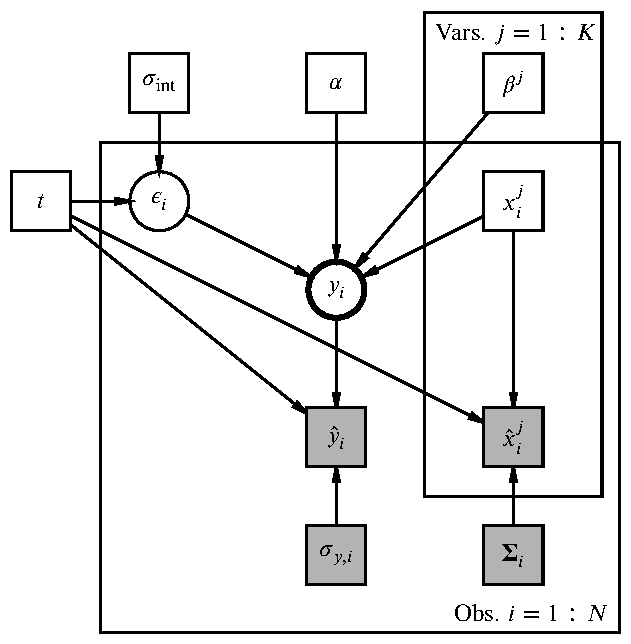
\includegraphics[width=\columnwidth]{graphics/dag.pdf}
    \caption{A directed acyclic graph representing the $t$-cup model for the
    function $f(\boldsymbol{x}; \boldsymbol{\theta}) = \alpha +
    \boldsymbol{\beta} \cdot \boldsymbol{x}_i$.}
    \label{fig:formalism.dag}
\end{figure}

\subsection{Priors}
\label{sec:formalism.prior}

To ensure that our model is generically applicable to astronomical linear
regression, we ensure that both independent and dependent quantities are scaled
to have zero mean and unit variance. This allows us to set generic priors on the
scaled intercept, gradients and scatter $\{\tilde{\intercept},
\tilde{\covariate}, \tilde{\sigma}_{\text{int}}\}$ that do not require rescaling for
different units or datasets (though these priors can be revised to incorporate
prior information).

Our priors on the regression parameters $\{\tilde{\intercept},
\tilde{\covariate}, \tilde{\sigma}_{\text{int}}\}$ are
\begin{align}
    \tilde{\intercept} \sim&\; \mathcal N(\mu = 0, \sigma = 3), \\
    \tilde{\covariate} \sim&\; \mathcal N(\mu = 0, \sigma = 3), \\
    \tilde{\sigma}_{\text{int}} \sim&\; {\color{red}\Gamma(2, 2)}.
\end{align}
The motivation behind the prior on $\tilde{\intercept}$ is that, as the data is
pre-scaled to have zero mean and the relationship between quantities is assumed
to be linear, we would expect the data to have zero intercept.  {\color{red}
There's not a particularly strong motivation behind the $\tilde{\covariate}$,
other than it's broad and symmetric. A more motivated prior would be
$\text{Cauchy}(0, 1)$, which is equivalent to a uniform prior on the angle the
line makes with the axis for $\dim x = 1$... but might overly weight a
regression for $\dim x \geq 2$, when we might want something uniform on the unit
sphere?} The prior on $\tilde{\sigma}_{\text{int}}$ is following the suggestion
of \citet{Chung:2015}, who demonstrate that a prior with density at
$\tilde{\sigma}_{\text{int}} = 0$ will lead to a prediction of no intrinsic
scatter in datasets where intrinsic scatter is present. The prior recommended in
their paper is {\color{red} $\Gamma(2, 2)$}; however, as we have pre-scaled our
data to have unit variance, we adopt a more concentrated prior.

The prior on the latent values of the independent quantities $\{\indepvars\}$ is
a Gaussian mixture model prior, similar to that used in \citet{Kelly:2007}.
While \citeauthor{Kelly:2007} infers the complete prior as part of the model, we
found that such a prior led to sampling issues as a result of the lack of
identifiability inherent in a multicomponent Gaussian mixture model. Therefore,
we use extreme deconvolution \citep{Bovy:2011} to estimate the parameters of a
Gaussian mixture model approximating the latent distribution of
$\{\indepvars\}$, and use these parameters for the prior.

The prior on the shape parameter $\nu$ is
\begin{align}
    \nu \sim&\; {\color{red}\text{Inv-}\Gamma(3, 10)};
\end{align}
this prior was chosen to balance flexibility (such that the model could
accommodate both heavily leptokurtic distributions --- e.g. the Cauchy
distribution --- and normally-distributed data) and sampling issues (as $\nu
\leftarrow \infty$, different values of $\nu$ become rapidly indistinguishable).
The reasoning behind this choice of prior is expanded upon in Appendix
\ref{sec:t-prior}.

The exact choice of prior for $\nu$ is unimportant, as the model is designed to
be robust to model misspecification; the only key element is that nu is allowed
to vary to accommodate both normal and heavy-tailed distributions. By virtue of
this, difficulties in sampling $\nu$ according to this prior distribution do not
invalidate the results of the model, as long as there is coverage at both small
and large values of $\nu$. In Section \ref{sec:results.t}, we shall discuss sampling issues in
greater detail.

\subsection{Asymptotic normality}
\label{sec:formalism.asymptotic}

{\color{green} For Daniel}

\subsection{Implementation}
\label{sec:formalism.implementation}

The model described in Section \ref{sec:formalism.model} is implemented in Stan
\citep{Stan}, which is used to draw samples via a HMC No U-Turn Sampler. The
implementation is packaged as $t$-cup, available as a Python
package\footnotemark.

For the purposes of comparison, we have also implemented a model that mirrors
the above structure, but uses normal distributions at each stage --- this model
is referred to as $n$-cup.

\footnotetext{\url{https://github.com/wm1995/tcup}}

\section{Validation}
\label{sec:methods}

In this section, we outline the methods used to validate the model set out in
the previous section. We run two types of tests to validate the performance of
$t$-cup under different types of model misspecification: simulation-based
calibration tests \citep{Cook:2006, Talts:2018} and fixed value calibration
tests.

\subsection{Simulation-based calibration}
\label{sec:methods.sbc}

Simulation-based calibration tests \citep{Cook:2006, Talts:2018} are used to
diagnose sampling issues. Parameters of interest $\theta_0$ are drawn from the
model prior $\pi(\theta)$, and a dataset is drawn following the prescription of
the model. We can then run a single MCMC chain on this dataset until we have
drawn $L$ independent samples $\{\tilde{\theta}_{i}\}$ (see \citet{Talts:2018}
for a discussion of independence criteria). We then compute the rank statistic
\begin{equation}
    r(\theta_0, \tilde{\boldsymbol{\theta}}_{\text{MCMC}})
        = \sum_{i = 1}^{L} \mathbb I [\tilde{\theta}_i < \theta_0].
\end{equation}
If the generative model matches the sampling model and the sampling algorithm
correctly draws samples from the posterior, the rank statistic will be uniformly
distributed across the integers $[0, L]$. We can, therefore, repeat this process
many times to build a histogram of rank statistics; any shortfalls in the
sampling algorithm will manifest as deviations from uniformity.

While this procedure has been developed to diagnose sampling issues, we can also
use the method to build a heuristic measure of how robust a model is to
misspecification. If the generative model and the sampling model no longer
match, we would expect deviations from uniformity in the rank statistic
histogram. We can compare how well different sampling models deal with model
misspecifcation by building the rank statistic histogram and assessing the
deviation from uniformity.

As our priors are defined in a scaled space, our simulation-based calibration
tests are also conducted in this scaled space; in this way, we are solely
testing the performance of the MCMC models, and not of the scaling before
fitting the models.

\subsection{Fixed-value calibration}
\label{sec:methods.fixed}

For our fixed-value calibration tests, we simulate datasets from known models
with true fixed values for our regression parameters. The purpose of these tests
is to demonstrate accurate recovery of these values, and to compare with the
results given when using normal distributions.

We generate multiple datasets with the same ground-truth parameters to verify
the results across multiple runs, producing plots of the cumulative distribution
function of the posterior medians calculated by the sampler. In each instance,
full specifications of the data models are specified in Appendix
\ref{sec:data-models}.

We aim to do a full end-to-end test of our inference pipeline in the fixed-value
calibration tests; therefore, these datasets are generated in the unscaled space
and are a test not only of the MCMC model but also of the scaling.

% Normally the next section describes the techniques the authors used.
% It is frequently split into subsections, such as Section~\ref{sec:maths} below.

% \subsection{Maths}
% \label{sec:maths} % used for referring to this section from elsewhere

% Simple mathematics can be inserted into the flow of the text e.g. $2\times3=6$
% or $v=220$\,km\,s$^{-1}$, but more complicated expressions should be entered
% as a numbered equation:

% \begin{equation}
%     x=\frac{-b$\pm$\sqrt{b^2-4ac}}{2a}.
% 	\label{eq:quadratic}
% \end{equation}

% Refer back to them as e.g. equation~(\ref{eq:quadratic}).

% \subsection{Figures and tables}

% Figures and tables should be placed at logical positions in the text. Don't
% worry about the exact layout, which will be handled by the publishers.

% Figures are referred to as e.g. Fig.~\ref{fig:example_figure}, and tables as
% e.g. Table~\ref{tab:example_table}.

\section{Results on simulated datasets}
\label{sec:results}

In the previous section, we proposed a general-purpose, robust statistical model
for linear regression; in this section, we investigate the performance of the
model on a series of simulated datasets with known parameters. Code that
reproduces the datasets in this section is available online\footnotemark.

\footnotetext{\url{https://github.com/wm1995/tcup-paper}}

\subsection{\textit{t}-distributed data}
\label{sec:results.t}

\begin{figure*}
    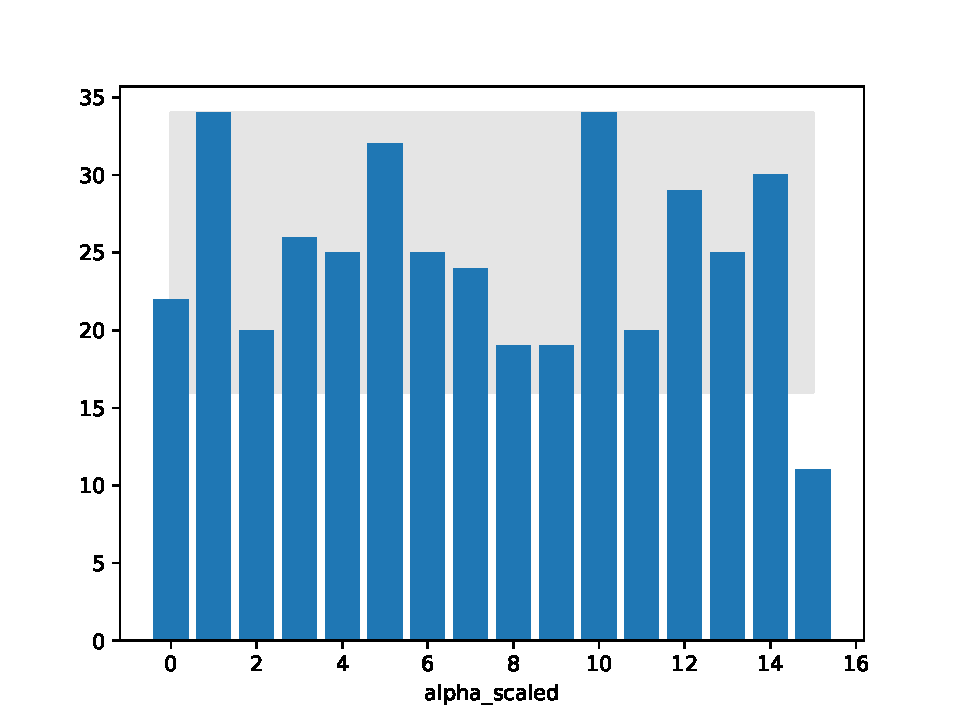
\includegraphics[width=0.19\textwidth]{graphics/sbc_t/alpha_scaled.pdf}
    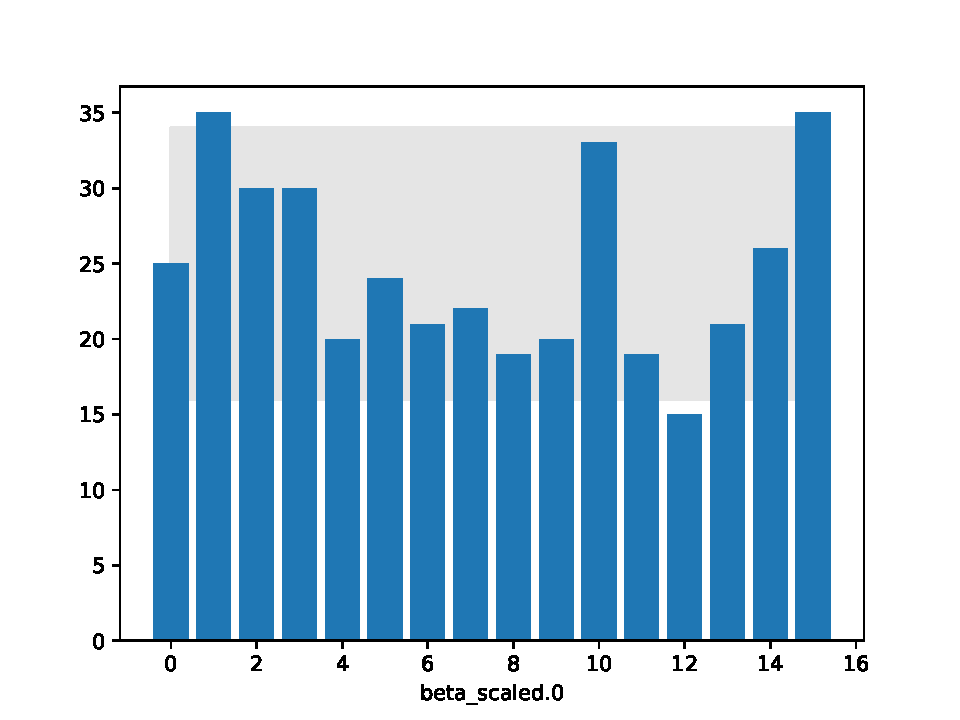
\includegraphics[width=0.19\textwidth]{graphics/sbc_t/beta_scaled.0.pdf}
    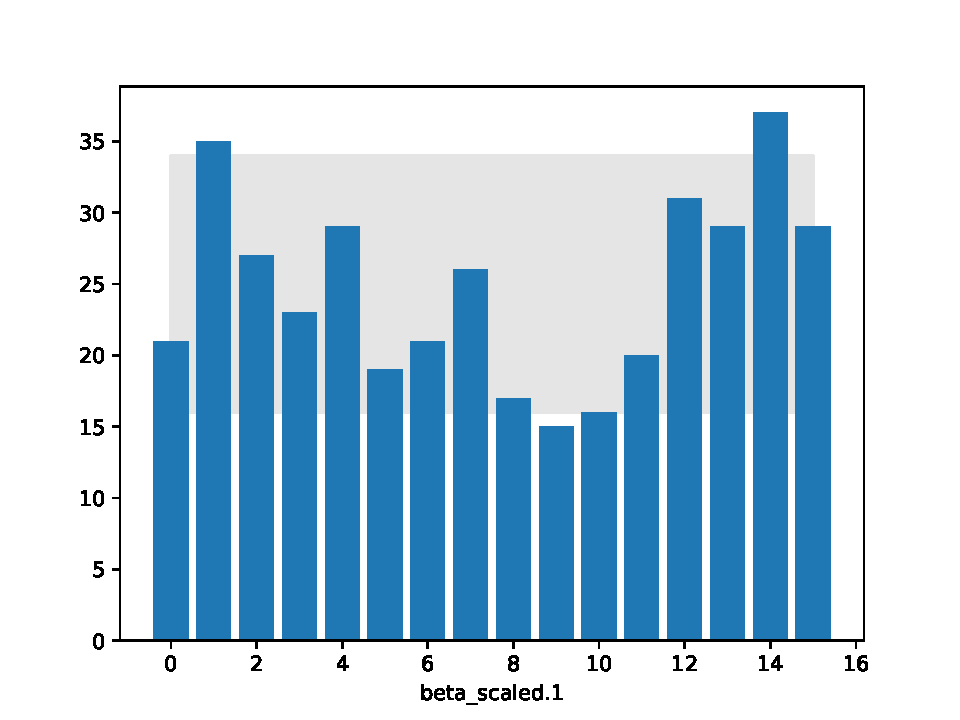
\includegraphics[width=0.19\textwidth]{graphics/sbc_t/beta_scaled.1.pdf}
    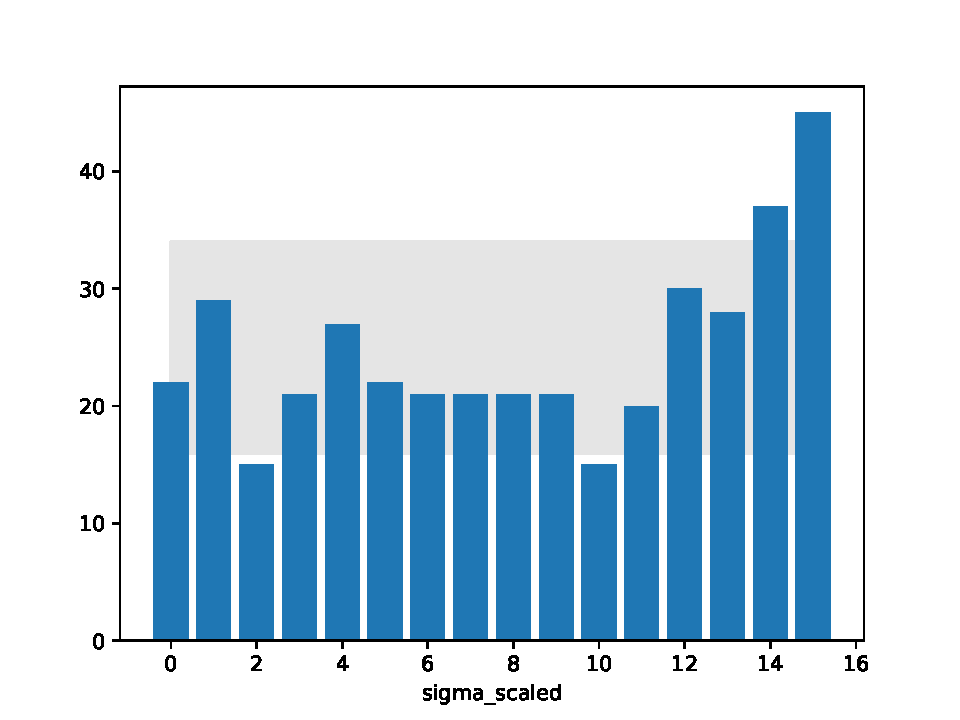
\includegraphics[width=0.19\textwidth]{graphics/sbc_t/sigma_scaled.pdf}
    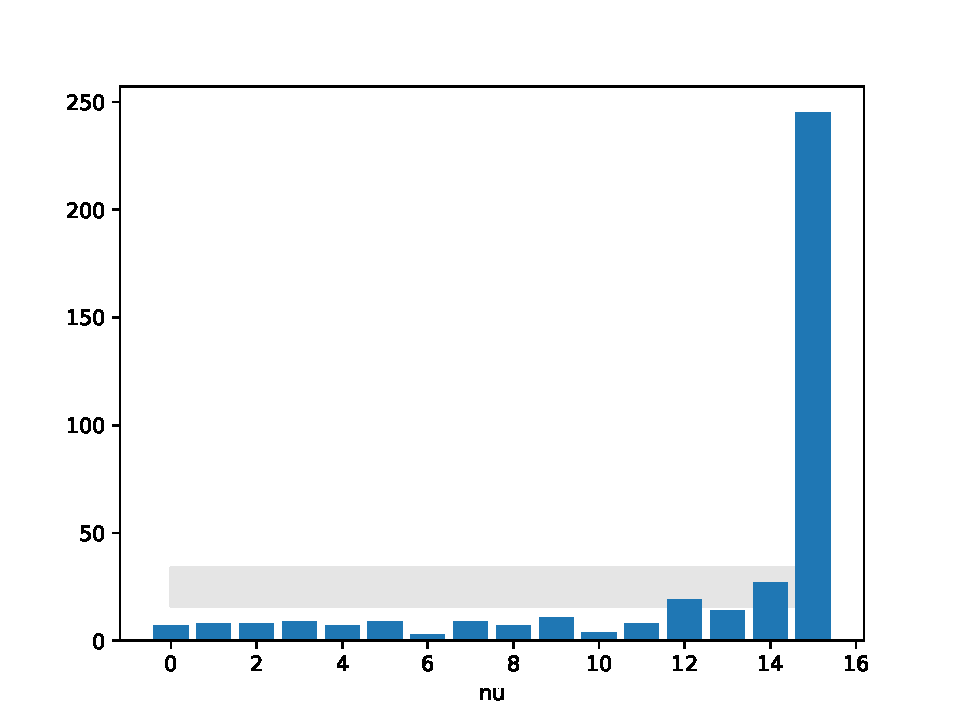
\includegraphics[width=0.19\textwidth]{graphics/sbc_t/nu.pdf}
    \caption{SBC runs for the t distribution under $t$-cup {\color{red} I know
    there are several tweaks needed to these plots}}
    \label{fig:results.t.sbc}
\end{figure*}

For our first test, we start with a dataset that matches our model perfectly
(i.e.\ $\mathcal P_{\text{int}} = \mathcal P_{\text{obs}} = t_\nu$). The
simulation-based calibration tests show that, while we are accurately inferring
$\alpha$ and $\boldsymbol{\beta}$, our inference for $\sigma_{int}$ and $\nu$ is
biased. The bias in $\nu$ arises because of the lack of identifiability for
larger values of $\nu$, which biases the MCMC estimates of $\nu$ to be lower
than the true values. The bias in $\sigma$ is a byproduct of this - if $\nu$ is
underestimated, then $\sigma$ will be underestimated as well.

For our fixed-value tests, we drew $N = 20$ datapoints with $\{\alpha, \beta,
\sigma_{\rm int}, \nu\} = \{3, 2, 0.1, 3\}$; the full model used to generate the
data is specified in Appendix \ref{sec:data-models.t}.


The chosen value of $\nu = 3$ corresponds to an outlier fraction of $\omega(\nu = 3)
\approx 5.8 \%$.

% \begin{figure}
%     \includegraphics[width=\columnwidth]{example-image-a}
%     \caption{{\color{red} 100} draws from the posterior of regression lines
%     (red) for the \textit{t}-distributed dataset (black points). The ground
%     truth regression line is illustrated by the black dashed line.}
%     \label{fig:results.t.regression}
% \end{figure}

\begin{figure}
    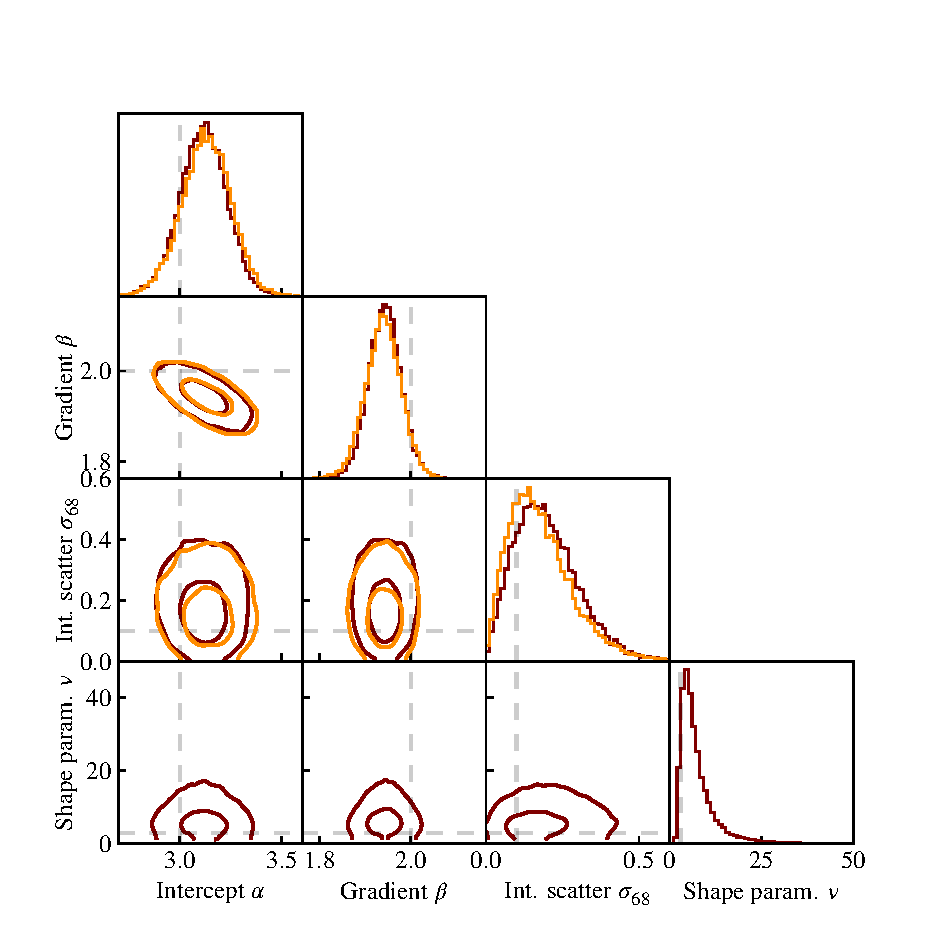
\includegraphics[width=\columnwidth]{graphics/corner_t.pdf}
    \caption{The posterior for each of the regression coefficients and the shape
    parameter $\nu$ for the \textit{t}-distributed dataset, with ground-truth
    values indicated by the black dashed lines. Contours indicate 39.3\% and
    86.5\% highest posterior density regions, corresponding to 1$\sigma$ and
    2$\sigma$ contours for a bivariate normal distribution.}
    \label{fig:results.t.corner}
\end{figure}

As we can see in Figures \ref{fig:results.t.regression} and
\ref{fig:results.t.corner}, we recover the values of the parameters that were
used to generate the dataset.

We then generated 1000 datasets from the same ground-truth parameters, and
calculated the maximum a posteriori (MAP) values of the regression coefficients
and shape parameter $\nu$. The results shown in Figure
\ref{fig:results.t.map} indicate that the estimate of true parameter values is
unbiased.{
\color{red} The true parameter values were contained in the 95\% highest
posterior density credible intervals $x$\% of the time across all parameters and
runs.
}

% \begin{figure}
%     \includegraphics[width=\columnwidth]{example-image-a}
%     \caption{The distribution of maximum a posteriori (MAP) estimates for each
%     of the regression parameters, as well as the shape parameter $\nu$.}
%     \label{fig:results.t.map}
% \end{figure}

\subsection{Normally-distributed data}
\label{sec:results.outlier}

\begin{figure*}
    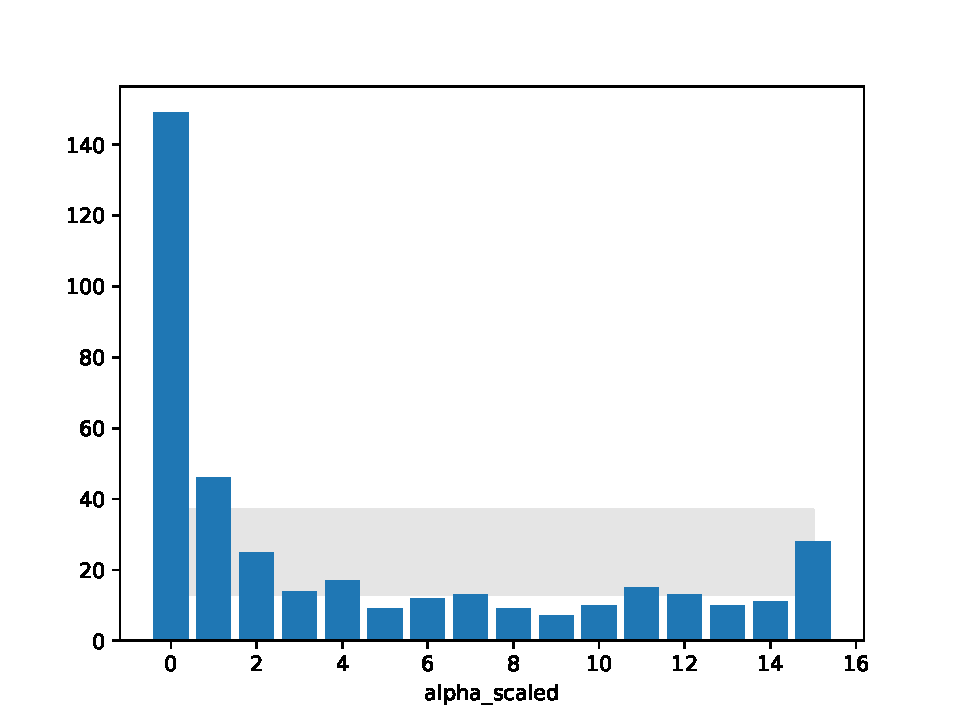
\includegraphics[width=0.24\textwidth]{graphics/sbc_outlier_ncup/alpha_scaled.pdf}
    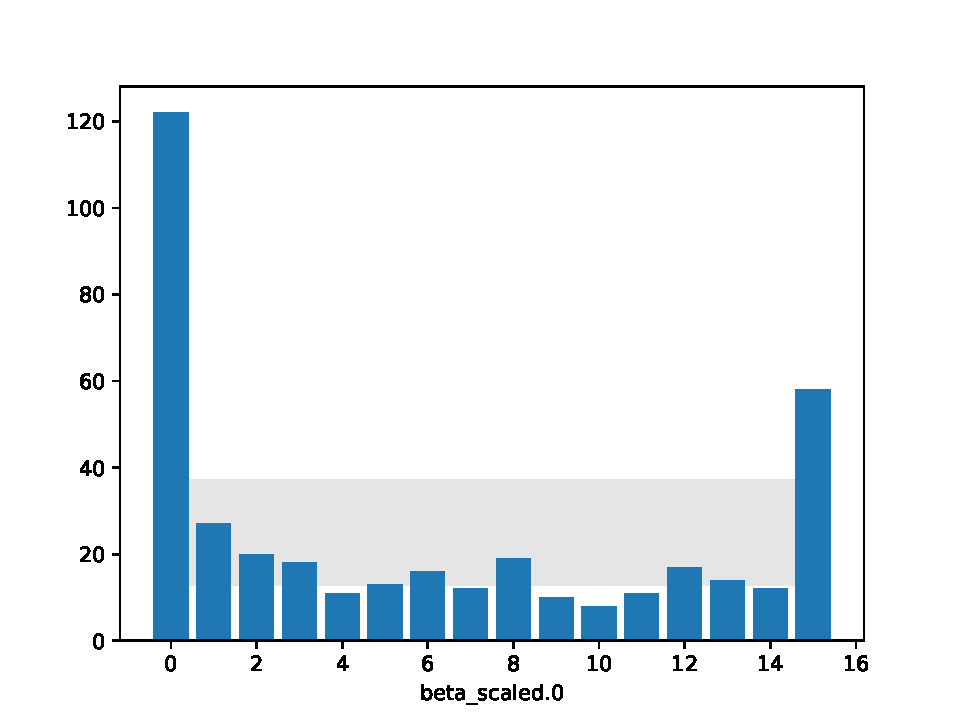
\includegraphics[width=0.24\textwidth]{graphics/sbc_outlier_ncup/beta_scaled.0.pdf}
    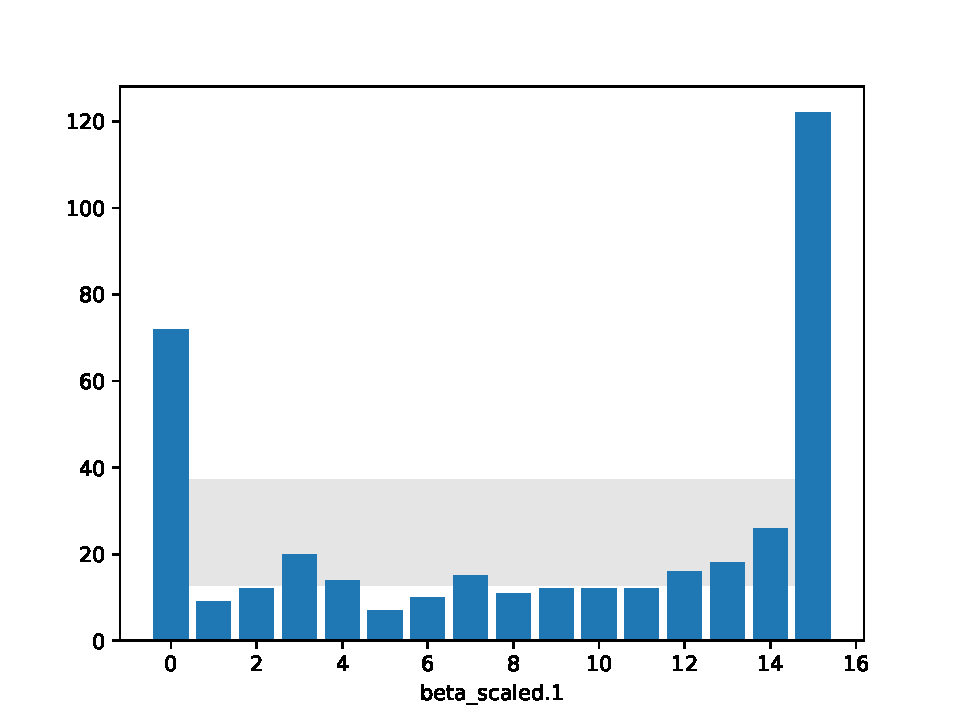
\includegraphics[width=0.24\textwidth]{graphics/sbc_outlier_ncup/beta_scaled.1.pdf}
    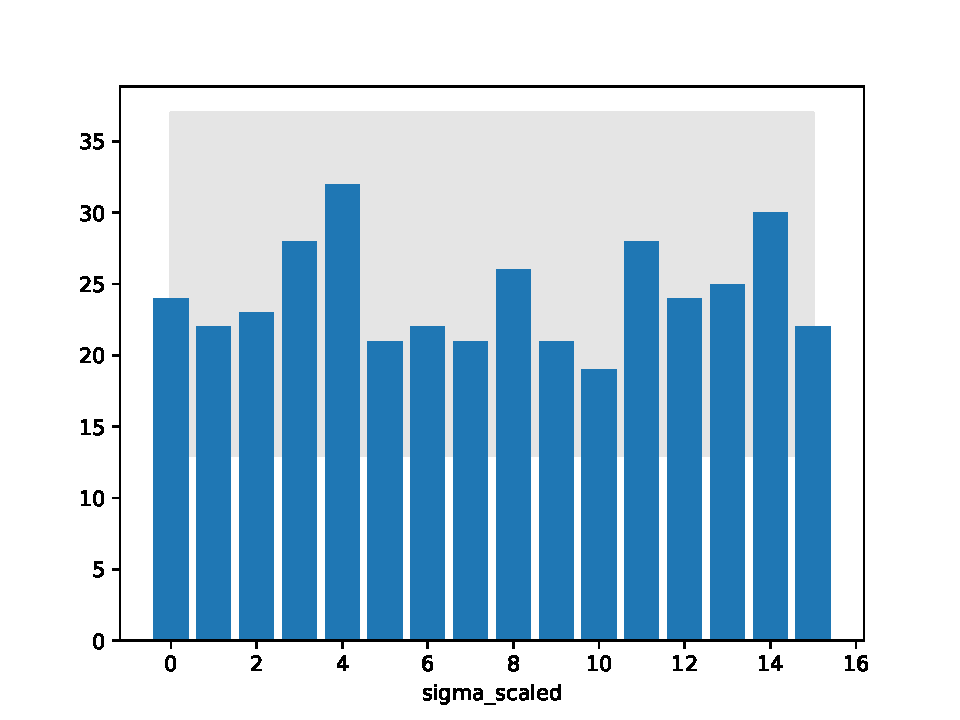
\includegraphics[width=0.24\textwidth]{graphics/sbc_outlier_ncup/sigma_scaled.pdf}
    \caption{SBC runs for the outlier dataset under $n$-cup {\color{red} I know
    there are several tweaks needed to these plots}}
    \label{fig:results.t.sbc}
\end{figure*}

\begin{figure*}
    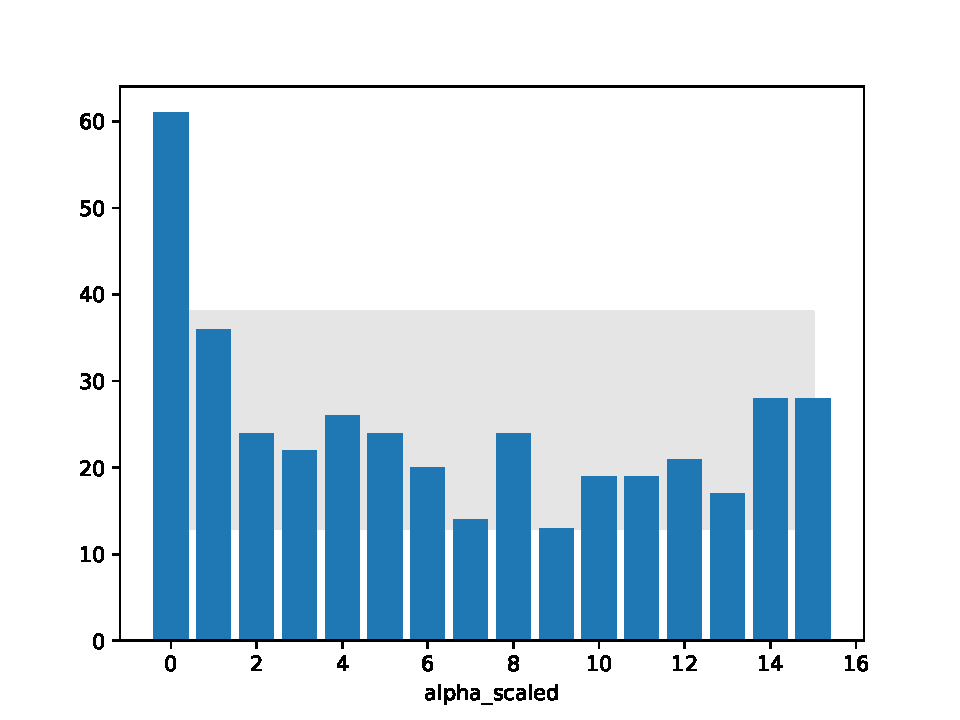
\includegraphics[width=0.24\textwidth]{graphics/sbc_outlier_tcup/alpha_scaled.pdf}
    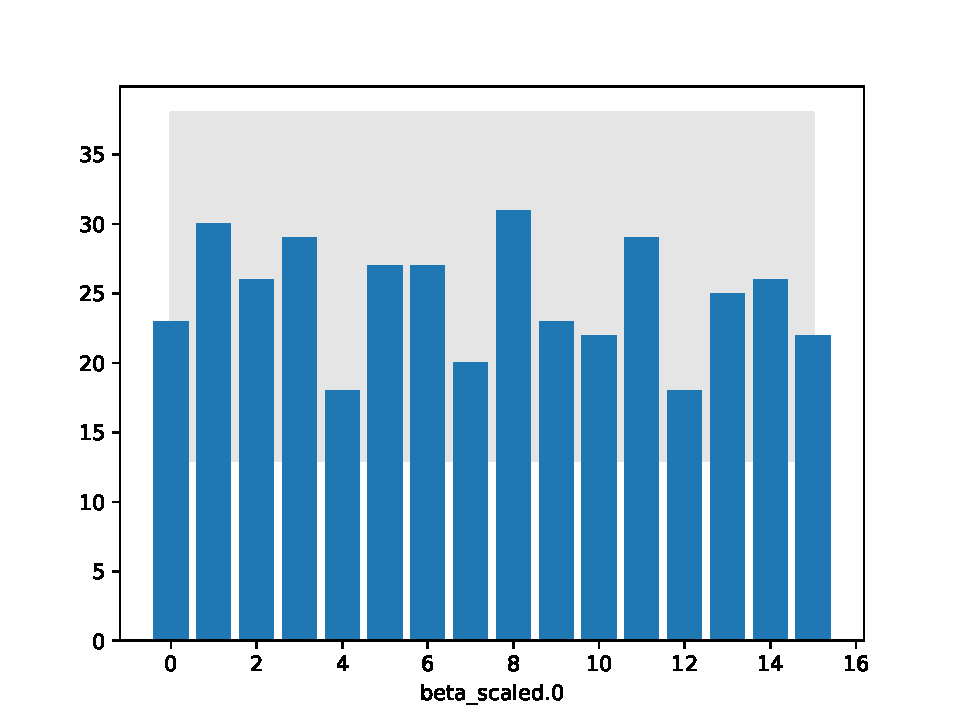
\includegraphics[width=0.24\textwidth]{graphics/sbc_outlier_tcup/beta_scaled.0.pdf}
    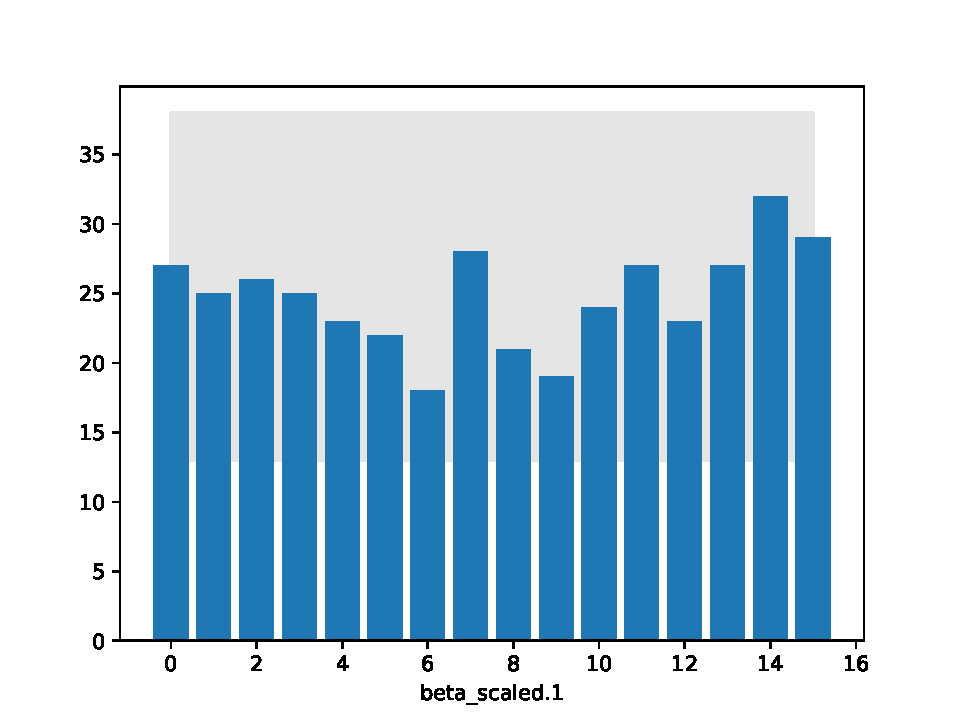
\includegraphics[width=0.24\textwidth]{graphics/sbc_outlier_tcup/beta_scaled.1.pdf}
    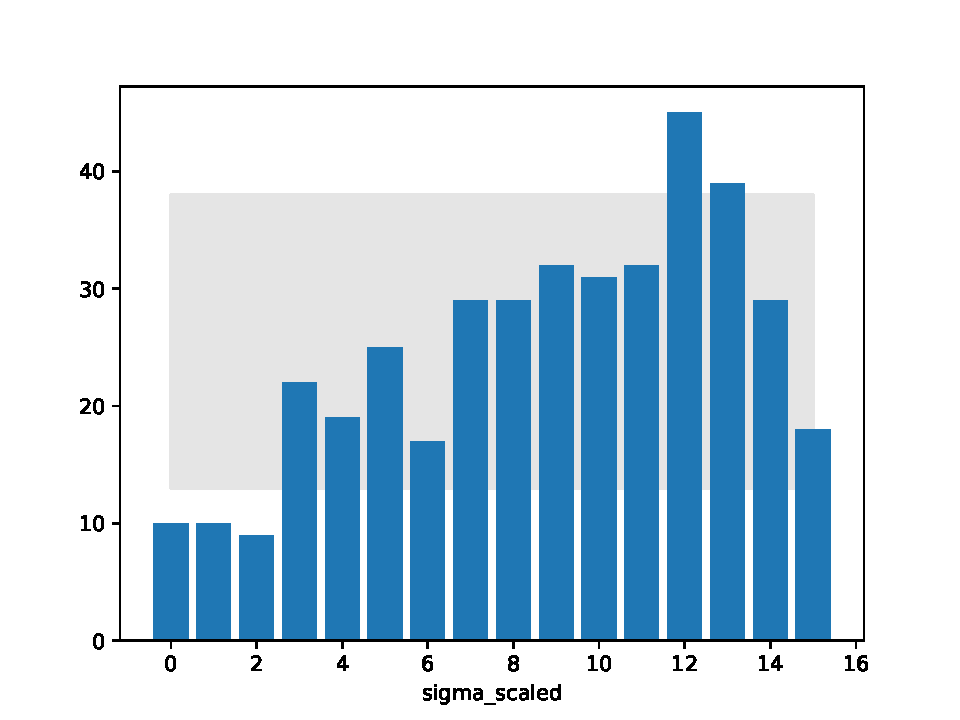
\includegraphics[width=0.24\textwidth]{graphics/sbc_outlier_tcup/sigma_scaled.pdf}
    \caption{SBC runs for the outlier dataset under $t$-cup {\color{red} I know
    there are several tweaks needed to these plots}}
    \label{fig:results.t.sbc}
\end{figure*}

In this test, we compare $t$-cup with an equivalent model that employs normal
distributions to illustrate that:
\begin{enumerate}
    \item $t$-cup is able to reduce to a normal model in the absence of outliers
    \item $t$-cup is able to give less biased results when an extreme outlier is
          introduced.
\end{enumerate}
A dataset of $N = 12$ points was generated with $\{\alpha, \beta, \sigma_{\rm
int}\} = \{3, 2, 0.2\}$, and one of the points was modified to be a
$\sim20~\sigma$ outlier (the full generative model is given in Appendix
\ref{sec:data-models.outlier}). While such an extreme outlier can easily be
spotted and removed, the purpose here is to demonstrate that $t$-cup does not
require this to give {\color{red} unbiased} estimates of the regression
parameters.

\begin{figure*}
    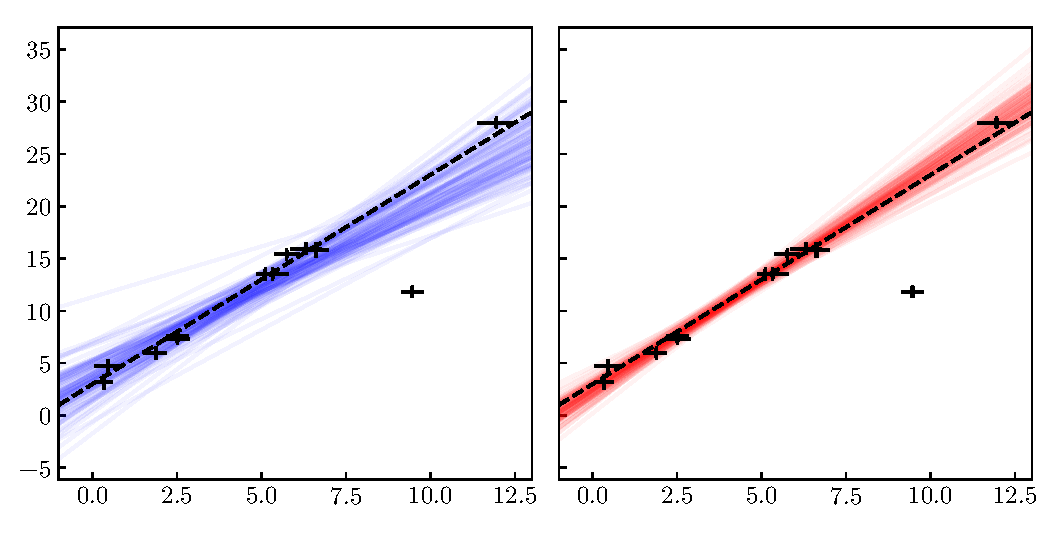
\includegraphics[width=\linewidth]{graphics/regression_outlier.pdf}
    \caption{{\color{red} 100} draws from the posterior of regression lines from
    the normal model (left panel, blue) and $t$-cup (right panel, red). The
    dataset is illustrated by the black points, with the ground-truth regression
    line illustrated by the black dashed line. {\color{red} I need to add axis
    labels to this figure - ``Observed $\hat{x}$'' and ``Observed $\hat{y}$''.}}
    \label{fig:results.outlier.regression}
\end{figure*}

\begin{figure}
    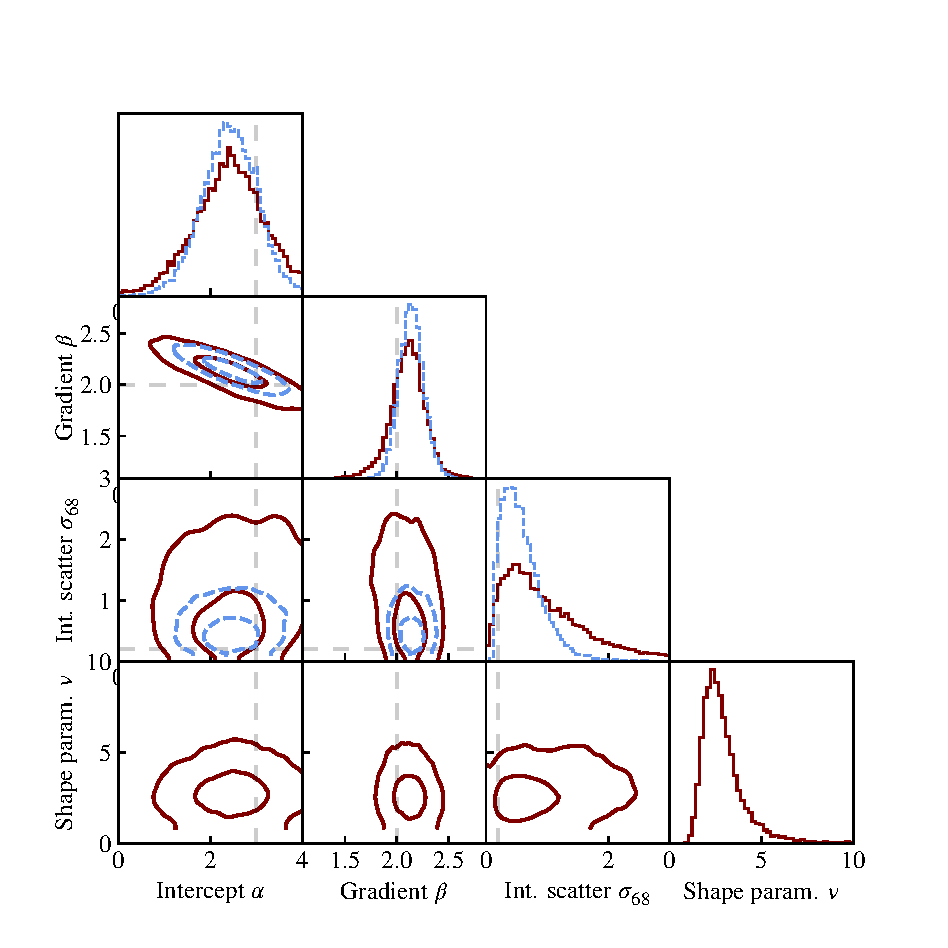
\includegraphics[width=\columnwidth]{graphics/corner_outlier_ncup.pdf}
    \caption{The posterior for each of the regression coefficients under the
    normal model with the outlier included (dark blue, solid) and excluded
    (light blue, dashed), and for $t$-cup with the outlier included (dark red,
    solid). Ground-truth values are indicated by the black dashed lines.}
    \label{fig:results.outlier.corner}
\end{figure}

\begin{figure}
    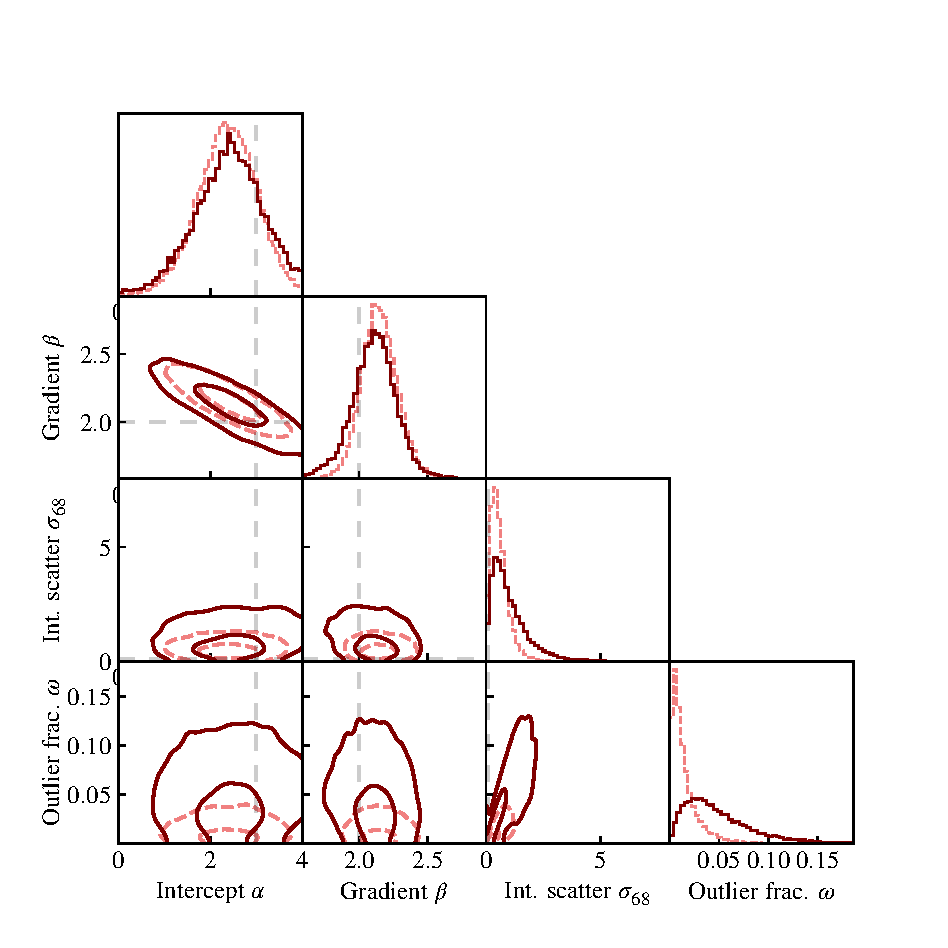
\includegraphics[width=\columnwidth]{graphics/corner_outlier_tcup.pdf}
    \caption{The posterior for each of the regression coefficients and the shape
    parameter $\nu$ under the $t$-cup model with the outlier included (dark red,
    solid) and excluded (light red, dashed). {\color{red} To do: fix contours
    that don't close at the bottom - I think this is an ArviZ issue.}}
    \label{fig:results.outlier.tcup}
\end{figure}

Figure \ref{fig:results.outlier.regression} illustrates how the estimates for
the true parameter models are biased in the normal model, but less affected in
the $t$-cup model.

In Figure \ref{fig:results.outlier.corner}, we compare the constraints on
parameters derived under the normal model (including and excluding the outlier
from the dataset), and the $t$-cup model (including the outlier only). The
constraints from the $t$-cup model including the outlier are consistent with
those derived under the normal model when the outlier is excluded, obviating the
need to remove the outlier manually. While this outlier is particularly extreme,
this example illustrates the utility of the $t$-cup model in datasets with
outliers.

For completeness, in Figure \ref{fig:results.outlier.tcup} we illustrate that
the $t$-cup model recovers consistent constraints whether the outlier is
included or excluded.

\begin{figure}
    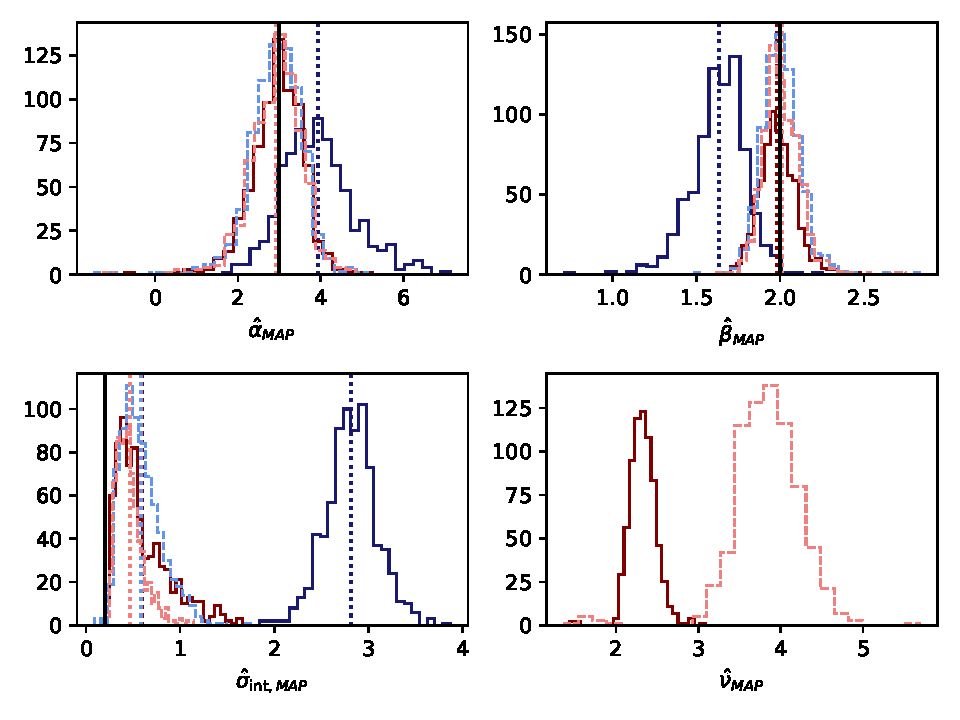
\includegraphics[width=\columnwidth]{graphics/outlier_many.pdf}
    \caption{The distribution of MAP estimates for each
    of the regression parameters under the normal model (blue) and $t$-cup model
    (red).}
    \label{fig:results.outlier.map}
\end{figure}

We then generated 1000 datasets using the same procedure, and calculated the
maximum a posteriori (MAP) values of the regression coefficients for both the
normal model and for $t$-cup. The results (illustrated in Figure
\ref{fig:results.outlier.map}) indicate that {\color{red} constraints under
$t$-cup are significantly less biased than those calculated under the normal
model. We also compared the 95\% highest-posterior density credible intervals
for each parameter,finding that the true parameter value was contained within
the interval for $x$\% of parameters and runs. }


\subsection{2D Normal Mixture Model with outlier fraction}
\label{sec:results.gmm}

This test is designed to further explore how $t$-cup performs when the model is
misspecified. In this case, we are looking at a normally-distributed population
which has a 10\% contamination rate with another normally-distributed population
of the same mean but 10 times the standard deviation. Equivalently, this test
can be thought of as investigating how the model performs when there is a
significant fraction of outliers.

The intrinsic scatter distribution $\mathcal P_{\rm int}$ is a mixture of two
normal distributions with zero mean; 90\% of points are drawn from a core
distribution with standard deviation $\sigma_\textrm{int}$, and 10\% of points
are drawn from an outlier distribution with standard deviation $10
\sigma_\textrm{int}$. The observation distribution $\mathcal P_{\rm obs}$ is a
normal distribution. For fixed-value tests, the true values of the regression
parameters were fixed to $\{\alpha, \beta_0, \beta_1, \sigma_{\rm int}\} = \{2,
3, 1, 0.4\}$. The full generative model for fixed-value tests is given in
Appendix \ref{sec:data-models.gmm}.

\begin{figure}
    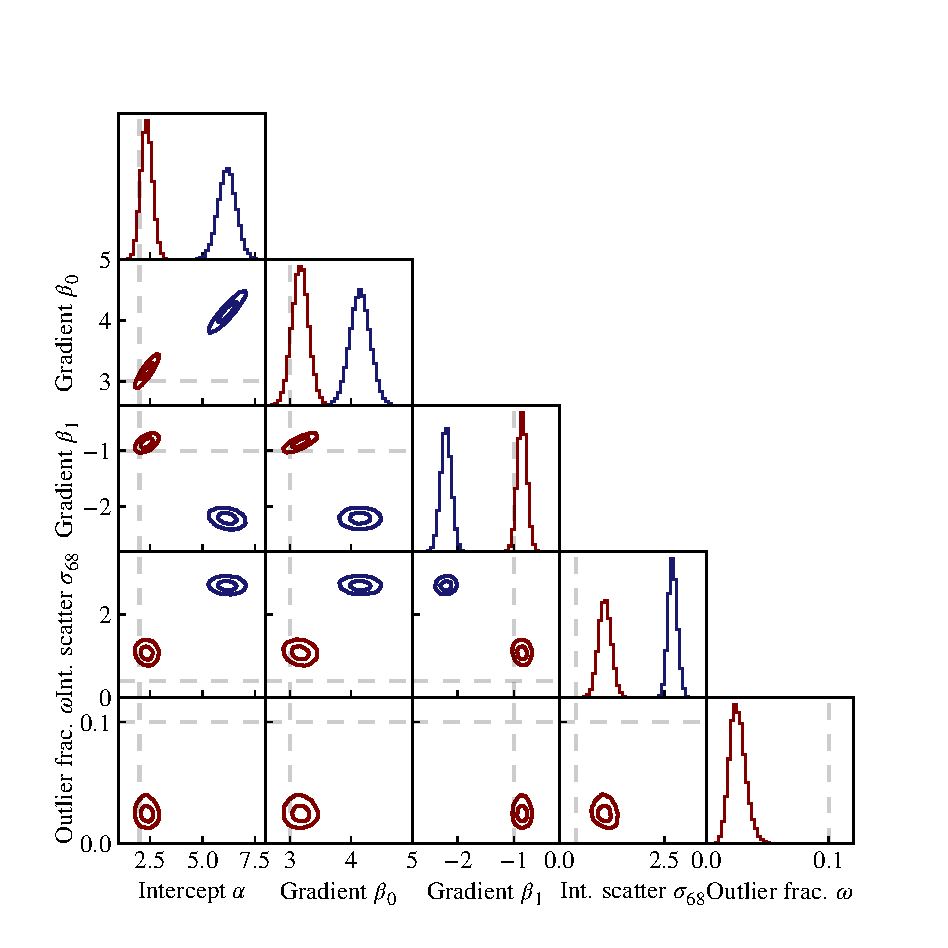
\includegraphics[width=\columnwidth]{graphics/corner_gaussian_mix.pdf}
    \caption{The posterior for each of the regression coefficients and the
    outlier fraction $\omega$ for the normal mixture model dataset, with
    ground-truth values indicated by the black dashed lines. {\color{red} To do:
    recalculate the outlier fraction shown on this plot - the $p = 0.1$ value
    (plotted) is not defined in the same way as outlier fraction $\omega$, so
    this isn't a fair comparison.}}
    \label{fig:results.gmm.corner}
\end{figure}

\subsection{Laplace-distributed data}
\label{sec:results.laplace}

For this test, we compare model performance on a symmetric, heavy-tailed, cuspy
distribution that does not fall into the family of $t$-distributions. Therefore,
we use a Laplace distribution as $\mathcal P_{\rm int}$, giving another example
of performance under explicit model misspecification.

We generate $N = 25$ datapoints from a model with Laplacian intrinsic scatter
(i.e.\ $\mathcal P_{\rm int} = \mathrm{Laplace}$) and normally distributed observation
noise (i.e.\ $\mathcal P_{\rm obs} = \mathcal N$). For the fixed-value tests, we
set $\{\alpha, \beta, \sigma_{\rm int}\} = \{-1, 0.8, 0.2\}$. The full
generative model can be found in Appendix \ref{sec:data-models.laplace}.

% \begin{figure}
%     \includegraphics[width=\columnwidth]{example-image-a}
%     \caption{{\color{red} 100} draws from the posterior of regression lines
%     (red) for the Laplace-distributed dataset (black points). The ground
%     truth regression line is illustrated by the black dashed line.}
%     \label{fig:results.laplace.regression}
% \end{figure}

% \begin{figure}
%     \includegraphics[width=\columnwidth]{example-image-a}
%     \caption{The posterior for each of the regression coefficients and the shape
%     parameter $\nu$ for the Laplace-distributed dataset, with ground-truth
%     values indicated by the black dashed lines.}
%     \label{fig:results.laplace.corner}
% \end{figure}

As we can see in Figures \ref{fig:results.laplace.regression} and
\ref{fig:results.laplace.corner}, we recover the values of the parameters that were
used to generate the dataset.

We then generated 1000 datasets from the same ground-truth parameters, and
calculated the maximum a posteriori (MAP) values of the regression coefficients
and shape parameter $\nu$. The results (illustrated in Figure
\ref{fig:results.laplace.map}) indicate that the estimate of true parameter
values is unbiased.{ \color{red} We also calculated the 95\% highest-posterior
density credible intervals for each parameter, finding that the true parameter
value was contained within the interval for $x$\% of parameters and runs.  }

% \begin{figure}
%     \includegraphics[width=\columnwidth]{example-image-a}
%     \caption{The distribution of maximum a posteriori (MAP) estimates for each
%     of the regression parameters, as well as the shape parameter $\nu$.}
%     \label{fig:results.laplace.map}
% \end{figure}


\subsection{Lognormally-distributed data}
\label{sec:results.lognormal}

For the final test in this section, we look at model performance for an
intrinsic scatter distribution that is asymmetric. For this reason, we choose
$\mathcal P_{\rm int}$ to be a lognormal distribution.

For the fixed-value datasets, generate $N = 25$ datapoints with $\{\alpha,
\beta\} = \{4, 8\}$; the full generative model is given in Appendix
\ref{sec:data-models.lognormal}.

% \begin{figure}
%     \includegraphics[width=\columnwidth]{example-image-a}
%     \caption{{\color{red} 100} draws from the posterior of regression lines
%     (red) for the lognormally-distributed dataset (black points). The ground
%     truth regression line is illustrated by the black dashed line.}
%     \label{fig:results.lognormal.regression}
% \end{figure}

% \begin{figure}
%     \includegraphics[width=\columnwidth]{example-image-a}
%     \caption{The posterior for each of the regression coefficients and the shape
%     parameter $\nu$ for the lognormally-distributed dataset, with ground-truth
%     values indicated by the black dashed lines.}
%     \label{fig:results.lognormal.corner}
% \end{figure}

As we can see in Figures \ref{fig:results.lognormal.regression} and
\ref{fig:results.lognormal.corner}, {\color{red} this needs to be rerun and
discussed.}

We then generated 1000 datasets from the same ground-truth parameters, and
calculated the maximum a posteriori (MAP) values of the regression coefficients
and shape parameter $\nu$. The results (illustrated in Figure
\ref{fig:results.lognormal.map}) indicate that the estimate of true parameter values is
unbiased.{
\color{red} We also calculated the 95\% credible intervals for each parameter,
finding that the true parameter value was contained within the interval for
$x$\% of parameters and runs.
}

% \begin{figure}
%     \includegraphics[width=\columnwidth]{example-image-a}
%     \caption{The distribution of maximum a posteriori (MAP) estimates for each
%     of the regression parameters, as well as the shape parameter $\nu$.}
%     \label{fig:results.lognormal.map}
% \end{figure}


\section{Demonstration on real data}
\label{sec:real-world}

% A simple demonstration on real data (Park is a possibility; another is an
% M-sigma analysis; possibly the data from the Kelly paper).  Suggest trying this
% on the paper used by Kelly as can directly compare.

Having seen $t$-cup's performance on simulated data in the previous section, we
now compare the performance of the $t$-cup model with a generic astronomical
Bayesian linear regression model \citep[\textsc{linmix\_err};][]{Kelly:2007} and
a tailored approach using $t$-distributions \citep{Park:2017}.

\subsection{\textsc{linmix\_err}}

We use the same dataset that is used in Section 8 of \citet{Kelly:2007} -- a
dataset of $N = 39$ quasars with measured Eddington ratio $L / L_{\text{Edd}}$
and X-ray spectral index $\Gamma$. Performance is compared with a Python
implementation\footnotemark of the original \textsc{linmix\_err} paper proposed
by \citeauthor{Kelly:2007}.

\footnotetext{https://github.com/jmeyers314/linmix}

\begin{table}
	\centering
	\caption{A comparison of estimates for the intercept,
    slope, and intrinsic scatter inferred for the relationship between Eddington
    ratio $L / L_{\text{Edd}}$ and X-ray spectral index $\Gamma$. The parameter
    estimates reported in \citet{Kelly:2007} are the posterior median and ``a
    robust estimate of the standard deviation''; for linmix and $t$-cup, we
    report the posterior median and an estimate of the standard deviation as
    $\sigma = 1.4826 MAD$.}
	\label{tab:real-world.kelly.params}
	\begin{tabular}{lccc} % four columns, alignment for each
                               & \citet{Kelly:2007} & linmix   & $t$-cup       \\
    Intercept $\alpha$         & 3.12 $\pm$ 0.41 & 3.18 $\pm$ 0.48 & 3.48 $\pm$ 0.35 \\
    Slope $\beta$              & 1.35 $\pm$ 0.54 & 1.40 $\pm$ 0.60 & 1.80 $\pm$ 0.44 \\
    Int. scatter $\sigma_{68}$ & 0.26 $\pm$ 0.11 & 0.25 $\pm$ 0.12 & 0.15 $\pm$ 0.09 \\
    Outlier fraction $\omega$  &      ---      &      ---      & 0.041 $\pm$ 0.025 \\
\end{tabular}
\end{table}

While the parameter estimates are broadly consistent (see Table
\ref{tab:real-world.kelly.params}), the posterior distributions in Figure
\ref{fig:real-world.kelly.corner} can be seen to differ, with the posterior
inferred by \textsc{linmix} being more diffuse than that inferred by $t$-cup.
The tighter constraints of $t$-cup suggest that the inference presented by
\citet{Kelly:2007} may biased by the assumption of normally-distributed data,
which may not hold true in this case.
The explicit assumption of normality in \textsc{linmix} is in tension with the
outlier fraction estimated by $t$-cup (68\% CI $\omega =
0.041^{+0.032}_{-0.021}$). This showcases that analysing data with robust
procedures gives materially different answers on real-world data, and highlights
the importance of carefully considering the implications when assuming
normality.

\begin{figure}
    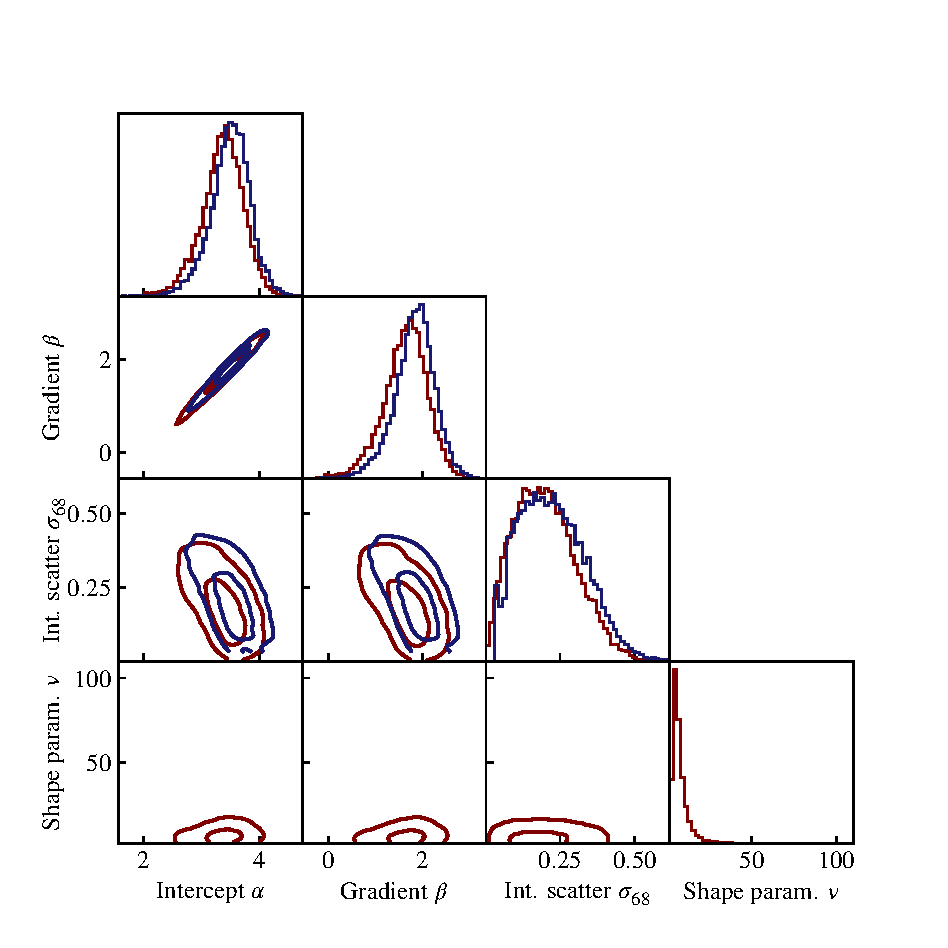
\includegraphics[width=\columnwidth]{graphics/corner_kelly.pdf}
    \caption{The posterior distributions for the data from \citet{Kelly:2007}
    under the linmix (blue) and $t$-cup (red) models.}
    \label{fig:real-world.kelly.corner}
\end{figure}

\subsection{\citet{Park:2017}}

This dataset consists of $N = 31$ AGN with reverberation-mapped mass estimates
$M_{\text{BH}}$, \textsc{Civ} emission line width $\Delta V$, and continuum
luminosity $\lambda L_{\lambda}$.

We recover constraints on the regression relation
\begin{equation}
    \log_{10} \left( \frac{M_{\text{BH}}}{10^8 M_\odot} \right) =
        \alpha +
        \beta_0 \log_{10} \left( \frac{\lambda L_{\lambda}}{10^{44} \text{erg s}^{-1}} \right) +
        \beta_1 \log_{10} \left( \frac{\Delta V}{10^3 \text{km s}^{-1}} \right)
\end{equation}
consistent with those of \citet{Park:2017} --- see Figure
\ref{fig:real-world.park.corner}. {\color{red} This needs rerunning with the
latest version of the code.}

\begin{figure}
    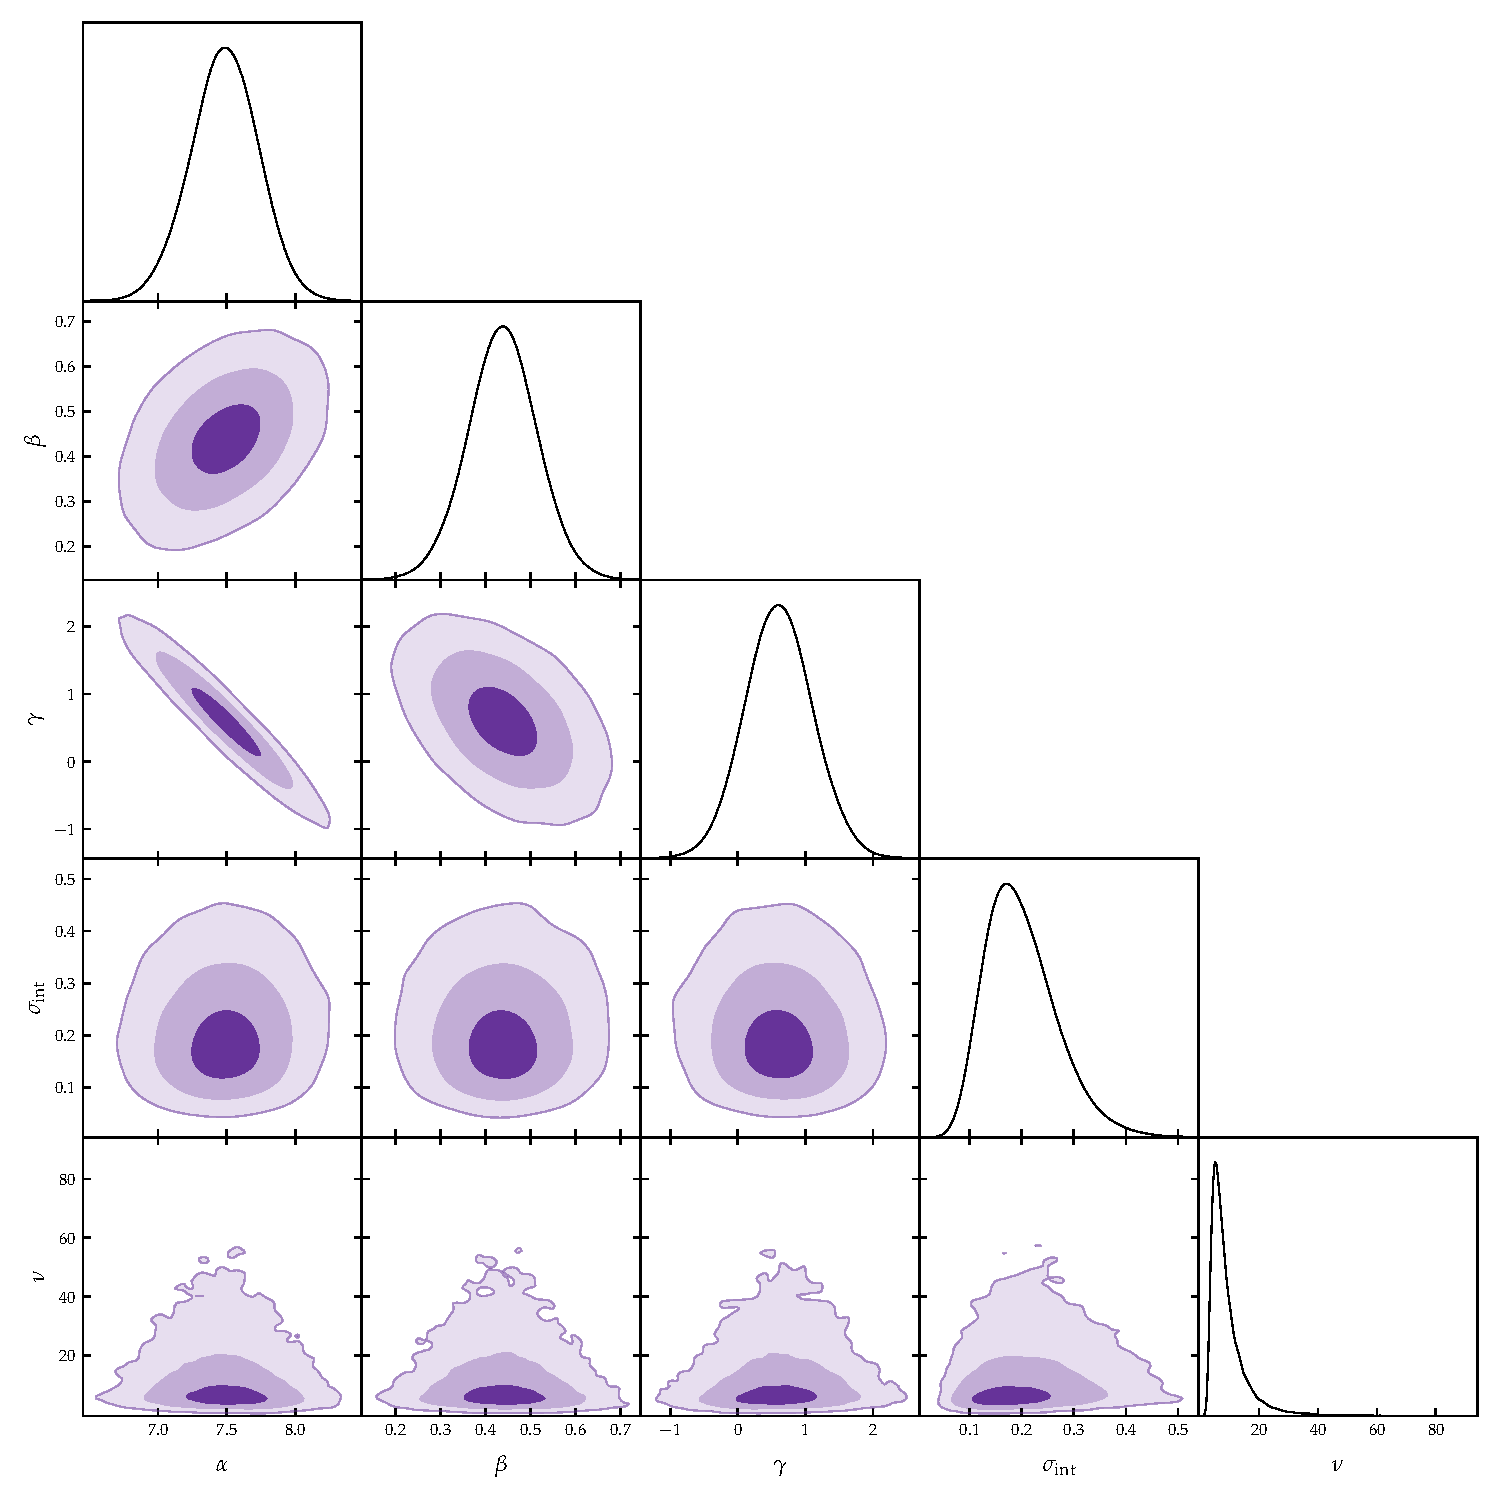
\includegraphics[width=\columnwidth]{graphics/corner_park.pdf}
    \caption{The posterior distributions for the data from \citet{Park:2007}
    under the $t$-cup model. {\color{red} This figure
    needs updating with the latest version of this model.}}
    \label{fig:real-world.park.corner}
\end{figure}

% % Example figure
% \begin{figure}
% 	% To include a figure from a file named example.*
% 	% Allowable file formats are eps or ps if compiling using latex
% 	% or pdf, png, jpg if compiling using pdflatex
% 	%\includegraphics[width=\columnwidth]{example}
%     Column width is \the\columnwidth.
%     Text width is \the\textwidth.
%     \caption{This is an example figure. Captions appear below each figure.
% 	Give enough detail for the reader to understand what they're looking at,
% 	but leave detailed discussion to the main body of the text.}
%     \label{fig:example_figure}
% \end{figure}

% \begin{figure*}
% 	% To include a figure from a file named example.*
% 	% Allowable file formats are eps or ps if compiling using latex
% 	% or pdf, png, jpg if compiling using pdflatex
% 	%\includegraphics[width=\columnwidth]{example}
%     \the\textwidth
%     \caption{This is an example figure. Captions appear below each figure.
% 	Give enough detail for the reader to understand what they're looking at,
% 	but leave detailed discussion to the main body of the text.}
%     \label{fig:example_widefigure}
% \end{figure*}

% % Example table
% \begin{table}
% 	\centering
% 	\caption{This is an example table. Captions appear above each table.
% 	Remember to define the quantities, symbols and units used.}
% 	\label{tab:example_table}
% 	\begin{tabular}{lccr} % four columns, alignment for each
% 		\hline
% 		A & B & C & D\\
% 		\hline
% 		1 & 2 & 3 & 4\\
% 		2 & 4 & 6 & 8\\
% 		3 & 5 & 7 & 9\\
% 		\hline
% 	\end{tabular}
% \end{table}


\section{Conclusions}
\label{sec:conclusion}

This paper has demonstrated a general-purpose approach to linear regression that
is robust to model misspecification, with a model laid out in Section
\ref{sec:formalism}. In Section \ref{sec:results}, we demonstrated that the
model recovers constraints consistent with those used to generate the datasets,
including in cases where there is a mismatch between the generative model used
to create the dataset and our regression model. In Section \ref{sec:real-world},
we compared the method to \textsc{linmix\_err} \citep{Kelly:2007} on real-world
data, illustrating that the models derive consistent constraints.

Summarise the take-home point that the method is a form of robust inference;
works on all sorts of outliers; then lead on to use in Paper 2 on the mass
ladder.

\section*{Acknowledgements}

The authors would like to thank Stephen Feeney, Boris Leistedt, Justin Alsing,
Tamas Budavari and Chad Schafer for useful conversations. WM is supported by
STFC grant ST/T506151/1.

%%%%%%%%%%%%%%%%%%%%%%%%%%%%%%%%%%%%%%%%%%%%%%%%%%
\section*{Data Availability}


The data in this paper is sourced from \citet{Kelly:2007, Park:2017}. Scripts to
generate the simulated datasets used to validate the model in Section
\ref{sec:results} are available from the GitHub repository for this paper, at
https://github.com/wm1995/tcup-paper.

%%%%%%%%%%%%%%%%%%%% REFERENCES %%%%%%%%%%%%%%%%%%

\bibliographystyle{mnras}
\bibliography{references}

%%%%%%%%%%%%%%%%%%%%%%%%%%%%%%%%%%%%%%%%%%%%%%%%%%

%%%%%%%%%%%%%%%%% APPENDICES %%%%%%%%%%%%%%%%%%%%%

\appendix

\section{Prior choice for shape parameter}
\label{sec:t-prior}

As our model relies on Student's $t$-distributions, we review notation and
priors used by previous works and justify our reasoning for our prior choice. It
can be informative to reparameterise the shape parameter $\nu$ in a few
different ways.

\citet{Feeney:2018} introduced the concept of the ``peak height ratio'' $t$ ---
the ratio of central peak height of a $t$-distribution with shape parameter $nu$
to that of a normal distribution. A normal distribution has, by definition,
$t(\nu = \infty) = 1$; a Cauchy distribution has $t(\nu = 1) = \sqrt{\frac2\pi}
\approx 0.80$. For general $\nu$, peak height ratio $t$ is
\begin{eqnarray}
    t(\nu) &=& \frac{
        \studentt{x = \mu; \mu}{\sigma}
    }{
        \mathcal N \left(x = \mu; \mu, \sigma \right)
    } \\
    &=& \sqrt{\frac{2}{\nu}} \;
    \frac{
        \Gamma\left(\frac{\nu + 1}{2}\right)
    }{
        \Gamma\left(\frac{\nu}{2}\right)
    }.
\end{eqnarray}
As shown in Figure \ref{fig:model.peak_height}, the behaviour of $t(\nu)$ is
highly non-linear, reflecting that, for $\nu \gtrsim 10$, the Student's
$t$-distribution rapidly approaches a normal distribution.

% \begin{figure}
%     \centering
%     \includegraphics{scripts/peak-height.pdf}
%     \caption{A plot of peak height ratio $t$ with varying shape parameter $\nu$}
%     \label{fig:model.peak_height}
% \end{figure}

As we are using the flexibility of Student's $t$-distributions to adapt to
datasets with outliers, it can also be useful to consider the outlier fraction
$\omega$. If we define outliers as any points lying more than $3\sigma$ from the
mean $\mu$, the outlier fraction is
\begin{eqnarray}
    \omega(\nu)
    &=& P\left(
        \left|x - \mu \right| > 3 \sigma \;
        \middle| \;
        x \sim \studentt{\mu}{\sigma}
    \right) \\
    &=& 2 F_\nu \left(\mu - 3 \sigma \right),
\end{eqnarray}
where $F_\nu(x)$ is the cumulative distribution function for Student's
$t$-distribution with shape parameter $\nu$. Figure \ref{fig:model.outlier_frac}
shows the relationship between outlier fraction $\omega$ and shape parameter
$\nu$, with $\omega \rightarrow 2.70 \times 10^{-3} $ in the limit of a normal
distribution, i.e., as $\nu \rightarrow \infty$. We would, therefore, expect
that approximately 1 in 370 datapoints would be outliers for data that follows a
normal distribution; for Cauchy-distributed data (i.e. $\nu = 1$),
we would expect every fifth datapoint to be an outlier.

% \begin{figure}
%     \centering
%     \includegraphics{scripts/outlier-frac.pdf}
%     \caption{Outlier fraction $\omega$ as a function of $\nu$ - for large $\nu$,
%     $\omega$ tends to the Gaussian limit value of $\omega \rightarrow 2.70
%     \times 10^{-3}$}
%     \label{fig:model.outlier_frac}
% \end{figure}

Using Student's $t$-distributions for Bayesian inference means that we have to
specify a prior on the shape parameter $\nu$. One approach is to adopt a fixed
value of $\nu$, which is equivalent to setting a Dirac delta function prior: a
common choice is $\nu = 4$ \citep[e.g.][]{Berger:1994, Gelman:2013}.  Another
approach is to adopt a more flexible approach by allowing $\nu$ to vary
\citep[e.g.][]{Juarez:2010, Park:2017, Feeney:2018}.

In \citet{Feeney:2018}, it is argued that, for common choices of prior, too
much prior density is placed on large values of $\nu$; to rectify this, they
propose a uniform prior on peak height $t \sim U\left(0, 1\right)$. As this
prior has no closed form derivative (a requirement for Hamiltonian Monte Carlo),
they approximate this with the prior
\begin{equation}
    \mathcal P\left(\nu\right) \propto
    \frac{
        \Theta(\nu)
    }{
        \left(
            \left(\frac{\nu}{\nu_0}\right)^{1 / (2 a)}
            + \left(\frac{\nu}{\nu_0}\right)^{2 / a}
        \right)^a
    }
\end{equation}
where $\Theta(\nu)$ is the Heaviside step function, and $\nu_0$ and $a$ are
constants with values $\sim 0.55$ and $\sim 1.2$ respectively.  One feature of
this prior is that it has significant density for $0 < \nu < 1$; in extreme
cases, this can correspond to outliers that are more than 100 orders of
magnitude larger than $\sigma$. In theory, these unphysical regions of parameter
space ought to be excluded during the process of inference. However, the use of
Hamiltonian Monte Carlo (HMC) in such cases can lead to divergences in the
sampling process or inefficient sampling as the sampler struggles with regions
of high curvature --- see the discussion of this phenomenon in
\citet{Neal:2003}.

Another possible prior is on outlier fraction $\omega$. It could be argued that
the term outlier loses its meaning when the majority of a dataset is composed of
so-called ``outliers''; therefore, a natural choice of prior might be a uniform
distribution ranging from the normally-distributed outlier fraction of
$\sim$0.00270 to this ``maximum'' outlier fraction of 0.5, corresponding to $\nu
\sim 0.302$. This still leads to large outliers (some of 8 orders of magnitude
for 100 draws from the distribution), which are unphysical and continue to
present difficulties when sampling with HMC.

To limit the number of unphysical outliers, we can instead limit the prior to
consider only distributions that are less heavy-tailed than the Cauchy
distribution --- i.e. all those with $\nu > 1$. This prior can be set on either
peak height $t$ or outlier fraction $\omega$.

% \begin{figure}
%     \centering
%     \includegraphics{scripts/scaled-peak-height.pdf}
%     \caption{Rescaled peak height $\tilde{t}$ as a function of $\nu$; also
%     illustrated is the approximation given in Equation \ref{eqn:model.t_approx}.
%     }
%     \label{fig:model.t_approx}
% \end{figure}

Works using the $t$-distributions for robust inference have used different
priors for the shape parameter $\nu$, which controls how heavy-tailed the
distribution is. Priors suggested include:
\begin{itemize}
    \item priors of the form $\nu \sim \text{Inv-}\Gamma(\alpha, \beta)$ for
          some $\left\{\alpha, \beta\right\}$ -- e.g.
          \citet{Juarez:2010} uses $\left\{\alpha = 2, \beta = 10\right\}$;
          \citet{Ding:2014} uses $\left\{\alpha = 1, \beta = 10\right\}$
    \item A uniform prior in $\frac1\nu \sim U(0, 1)$ \citep{Gelman:2013}
    \item A uniform prior in distribution peak height relative to a normal
    distribution, such that
    \begin{equation}
        \sqrt{\frac2\nu}\frac{\Gamma\left(\frac{\nu + 1}{2}\right)}{\Gamma\left(\frac{\nu}{2}\right)} \sim U(0, 1).
    \end{equation}
\end{itemize}
These priors are illustrated in Figure \ref{fig:priors.pdf}.

\begin{figure}
	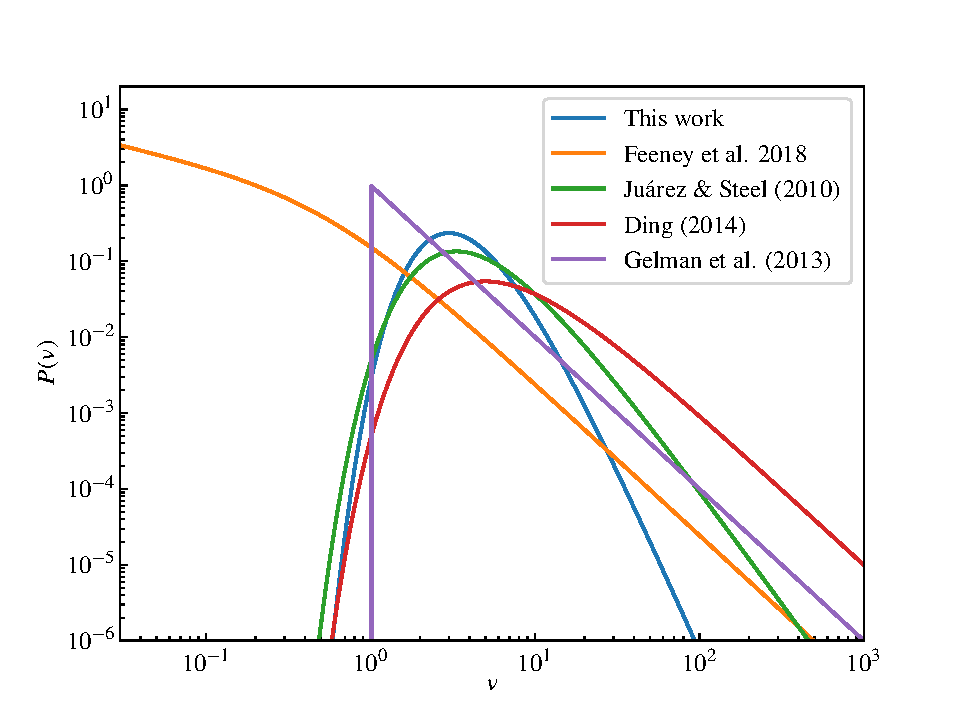
\includegraphics[width=\columnwidth]{graphics/pdf_nu}
    \caption{A selection of different priors on $\nu$ in works that have used
    $t$-distributions.}
    \label{fig:priors.pdf}
\end{figure}

A uniform proper prior in $\frac1\nu$ gives a hard cutoff in $\nu$, which
renders regions of parameter space inaccessible (in the case of the
\citet{Gelman:2013} prior, $\nu = 1$ is the cutoff, which corresponds to a
Cauchy distribution.) On the other hand, the prior used in \citet{Feeney:2018}
has disproportionate prior density at low values of $\nu$, which corresponds to
models with outliers several orders of magnitude larger than the predicted
effect size.

It can also be instructive to calculate the ``outlier fraction'' for different
values of $\nu$. We define the outlier fraction $\omega$ as
\begin{eqnarray}
    \omega(\nu) &=& \mathcal P\left(|x - \mu| > 3 \sigma \mid x \sim t_\nu (\mu, \sigma^2) \right) \\
    &=& I\left(\frac{\nu}{\nu + 3^2};\frac\nu2, \frac12\right),
\end{eqnarray}
where $I(x; \alpha, \beta)$ is the regularised beta function. For a normal
distribution, we expect about 0.27\% of points to be outliers greater than
3~$\sigma$ from the mean --- i.e. $\lim_{\nu \rightarrow \infty}\omega(\nu)
\approx 0.0027$; for a Cauchy distribution, $\omega(\nu = 1) \approx 0.20$.

The cumulative distribution functions for the priors in terms of outlier
fraction are illustrated in Figure \ref{fig:priors.outlier_frac}.
\begin{figure}
	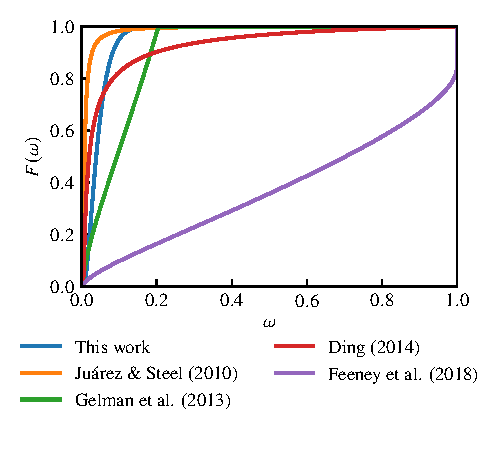
\includegraphics[width=\columnwidth]{graphics/cdf_outlier_frac}
    \caption{The CDF of priors on $\nu$ used in works that have used
    $t$-distributions. The priors are expressed in terms of outlier fraction
    $\omega$, which is the fraction of points in the distribution lying more
    than 3$\sigma$ from the mean.}
    \label{fig:priors.outlier_frac}
\end{figure}

In this work, we use the prior
\begin{equation}
    \nu \sim \text{Inv-}\Gamma(3, 10),
\end{equation}
where $\text{Inv-}\Gamma(\alpha, \beta)$ is an inverse gamma distribution with
{\color{red} shape parameter $\alpha$ and scale parameter $\beta$}.

This prior was chosen for two reasons:
\begin{itemize}
    \item the prior is smooth in $\nu$ with no sharp boundaries (unlike
          \citet{Gelman:2013})
    \item the prior has density at a larger range of outlier fractions $\omega$
          than those in \citet{Juarez:2010, Ding:2014} but insignificant density
          at unrealistically high outlier fractions, in contrast with the prior
          in \citet{Feeney:2018}.
\end{itemize}

\section{Fixed-value calibration data models}
\label{sec:data-models}

In this section, we fully specify the dataset models used for fixed-value
calibration tests in Section \ref{sec:results}.

\subsection{\textit{t}-distributed data}
\label{sec:data-models.t}

The fixed-value test datasets have $N = 20$ datapoints drawn from the following
distribution:
\begin{align}
    x_i \sim&\; \mathcal N (\mu = 2, \sigma = 2) \\
    y_i \sim&\; t_{3} (\mu = 3 + 2 x_i, \sigma = 0.1) \\
    \log_{10} \sigma_{x, i} \sim&\; \mathcal N (\mu = -1, \sigma = 0.1) \\
    \log_{10} \sigma_{y, i} \sim&\; \mathcal N (\mu = -0.7, \sigma = 0.1) \\
    \hat{x}_i \sim&\; t_{3} (\mu = x_i, \sigma = \sigma_{x, i}) \\
    \hat{y}_i \sim&\; t_{3} (\mu = y_i, \sigma = \sigma_{y, i}).
\end{align}

\subsection{Normally-distributed data with an outlier}
\label{sec:data-models.outlier}

We generated datasets of $N = 12$ points using the model:
\begin{alignat}{1}
    x_i& \sim \mathcal N (\mu = 5, \sigma = 3) \\
    y_i& \sim
    \begin{cases}
        \mathcal N (\mu = 3 + 2 x_i - 10, \sigma = 0.2) &
            \text{for the second-largest $x_i$} \\
        \mathcal N (\mu = 3 + 2 x_i, \sigma = 0.2) &
            \text{otherwise} \\
    \end{cases}\\
    \log_{10} \sigma_{x, i}& \sim \mathcal N (\mu = -0.5, \sigma = 0.1) \\
    \log_{10} \sigma_{y, i}& \sim \mathcal N (\mu = -0.3, \sigma = 0.1) \\
    \hat{x}_i& \sim \mathcal N (\mu = x_i, \sigma = \sigma_{x, i}) \\
    \hat{y}_i& \sim \mathcal N (\mu = y_i, \sigma = \sigma_{y, i}).
\end{alignat}

\subsection{2D Normal Mixture Model}
\label{sec:data-models.gmm}

We introduce the parameter $O_i$ to indicate whether the $i$th datapoint is
drawn from the core distribution (in which case, $O_i = 0$) or from the outlier
distribution (for which $O_i = 1$).

We generated a dataset of $N = 200$ points using the model:
\begin{alignat}{1}
    \boldsymbol{x}_i& \sim
    \begin{cases}
        \mathcal N \left(
            \mu = \begin{pmatrix} -3 \\ 2 \end{pmatrix},
            \sigma = \begin{pmatrix} 0.5 & -1 \\ -1 & 4 \end{pmatrix}
        \right) &
            1 \leqslant i \leqslant 140 \\
        \mathcal N \left(
            \mu = \begin{pmatrix} -1 \\ -1 \end{pmatrix},
            \sigma = \begin{pmatrix} 1 & 0.2 \\ 0.2 & 0.8 \end{pmatrix}
        \right) &
            140 < i \leqslant 200 \\
    \end{cases}\\
    O_i& \sim \mathrm{Bernoulli}(0.1) \\
    y_i& \sim
    \begin{cases}
        \mathcal N (\mu = 2 + (3, 1)^T \cdot x_i, \sigma = 0.4) &
            O_i = 0 \\
        \mathcal N (\mu = 2 + (3, 1)^T \cdot x_i, \sigma = 4.0) &
            O_i = 1 \\
    \end{cases}\\
    \Sigma_{x, i}& \sim \mathcal W_2 (\boldsymbol{V} = 0.1 \mathbb{I}, n = 3) \\
    \log_{10} \sigma_{y, i}& \sim \mathcal N (\mu = -1, \sigma = 0.1) \\
    \hat{x}_i& \sim \mathcal N (\mu = \boldsymbol{x}_i, \sigma = \Sigma_{x, i}) \\
    \hat{y}_i& \sim \mathcal N (\mu = y_i, \sigma = \sigma_{y, i}).
\end{alignat}

\subsection{Laplace-distributed data}
\label{sec:data-models.laplace}

We generate $N = 25$ datapoints under the following model:
\begin{eqnarray}
    x_i &\sim& \mathcal U (-5, 5) \\
    y_i &\sim& \mathrm{Laplace} (\mu = -1 + 0.8 x_i, b = 0.2) \\
    \log_{10} \sigma_{x, i} &\sim& \mathcal N (\mu = -1, \sigma = 0.1) \\
    \log_{10} \sigma_{y, i} &\sim& \mathcal N (\mu = -1, \sigma = 0.1) \\
    \hat{x}_i &\sim& \mathcal N (\mu = x_i, \sigma = \sigma_{x, i}) \\
    \hat{y}_i &\sim& \mathcal N (\mu = y_i, \sigma = \sigma_{y, i}).
\end{eqnarray}

\subsection{Lognormally-distributed data}
\label{sec:data-models.lognormal}

We generate $N = 25$ datapoints under the following model:
\begin{eqnarray}
    x_i &\sim& \mathcal U (-5, 5) \\
    \log_{10} y_i &\sim& \mathcal N (\mu = \log_{10} (4 + 8 x_i), \sigma = 0.2) \\
    \log_{10} \sigma_{x, i} &\sim& \mathcal N (\mu = -1, \sigma = 0.1) \\
    \log_{10} \sigma_{y, i} &\sim& \mathcal N (\mu = -1, \sigma = 0.1) \\
    \hat{x}_i &\sim& \mathcal N (\mu = x_i, \sigma = \sigma_{x, i}) \\
    \hat{y}_i &\sim& \mathcal N (\mu = y_i, \sigma = \sigma_{y, i}).
\end{eqnarray}


%%%%%%%%%%%%%%%%%%%%%%%%%%%%%%%%%%%%%%%%%%%%%%%%%%


% Don't change these lines
\bsp	% typesetting comment
\label{lastpage}
\end{document}

% End of mnras_template.tex
